%! Author = arqfa
%! Date = 8/8/2023


%!Document class for final manuscript
\documentclass[final,5p,times]{elsarticle}% Turn on the 'final' option to hide all changes and produce a clean output

%!document class for changes tracking
%\documentclass[5p,times]{elsarticle}% turn on for changes
%! package for tracking changes

\usepackage[final]{changes} %Turn on the 'final' option to hide all changes and produce a clean output
%\usepackage{changes}% turn on when going for manuscript with changes

    %% Added Text: Use \added{new text} to indicate added text.
    %Deleted Text: Use \deleted{old text} for text you have removed.
    %Replaced Text: Use \replaced{new text}{old text} to show text that has been replaced.

%% For including figures, graphicx.sty has been loaded in
%% elsarticle.cls.


%!Packages
%% The amssymb package provides various useful mathematical symbols
\usepackage{amssymb}
%% The amsthm package provides extended theorem environments
\usepackage{amsthm}
\usepackage{graphicx}
\usepackage{tabularx}
\usepackage{booktabs}
\usepackage{amsmath} % for equations
\usepackage{breakurl}
\usepackage{hyperref} % Ensure hyperlinks work properly


%% The lineno packages adds line numbers. Start line numbering with
%%\begin{linenumbers}, end it with \end{linenumbers}. Or switch it on
%% for the whole article with \linenumbers
\usepackage{lineno}
\modulolinenumbers[10]
\usepackage{enumitem}

%\usepackage{amsmath}

\usepackage{multirow}

\usepackage{caption}

\journal{Automation in Construction}


% Document
\begin{document}

\begin{frontmatter}


\title{Embracing Complexity: Virtual Reality Assessment of User Tolerance for Complex Facades in Future Construction Trends}

%% use optional labels to link authors explicitly to addresses:
%% \author[label1,label2]{}
%% \affiliation[label1]{organization={},
%%             addressline={},
%%             city={},
%%             postcode={},
%%             state={},
%%             country={}}
%%
%% \affiliation[label2]{organization={},
%%             addressline={},
%%             city={},
%%             postcode={},
%%             state={},
%%             country={}}

\author[inst1]{Fabian Jarrin}
\author[inst2]{Yasuko Koga}
\author[inst3]{Diego Thomas}

\affiliation[inst1]{organization={Graduate School of Human-Environment Studies, Department of Architecture, Kyushu University},%Department and Organization
            addressline={744 Motooka, Nishi-ku},
            city={Fukuoka},
            postcode={819-0395},
            %state={Fukuoka},
            country={Japan}}

\affiliation[inst2]{organization={Faculty of Human-Environment Studies, Department of Architecture and Urban Design, Kyushu University},%Department and Organization
            addressline={744 Motooka, Nishi-ku},
            city={Fukuoka},
            postcode={819-0395},
            %state={Fukuoka},
            country={Japan}}

\affiliation[inst3]{organization={Faculty of Information Science and Electrical Engineering, Department of Advanced Information Technology, Kyushu University},%Department and Organization
            addressline={744 Motooka, Nishi-ku},
            city={Fukuoka},
            postcode={819-0395},
            %state={Fukuoka},
            country={Japan}}



\begin{abstract}
%% Text of abstract
%!Asbtract guidelines
        %A concise and factual abstract (100-150 words ) is required. The abstract should state briefly the purpose of the research, the principal results and major conclusions. An abstract is often presented separately from the article, so it must be able to stand alone. For this reason, References should be avoided, but if essential, then cite the author(s) and year(s). Also, non-standard or uncommon abbreviations should be avoided, but if essential they must be defined at their first mention in the abstract itself.



% check
% new version under reviewer guidelines: Abstracts should contain only 6 short sentences: 1) What is the problem being addressed? 2) What is the research question being asked? 3) What is the methodology being used to answer the stated research question? 4) What are the results obtained? 5) What is the meaning and importance of these results? 6) What are the directions for follow-up research?


Architectural practice is evolving through digital fabrication, enabling complex designs that challenge the uniformity of barren walls and fully glazed facades that often dominate contemporary streetscapes.
This study investigates user tolerance and acceptance of complex facades using Virtual Reality (VR) and Computer Vision through the Computational Image Complexity Analysis (CICA) system.
We applied VR simulations and CICA to quantitatively and qualitatively assess reactions to various facade complexities.
Results reveal a preference for moderate complexity, suggesting an ideal balance between simplicity and intricacy.
This highlights the importance of aligning architectural complexity with user preferences to enhance sustainability and satisfaction.
Future research should explore the long-term impact of complex facades on user well-being and environmental sustainability.


%version 2024/05
%This research uses virtual reality (VR) assessment and computer vision to explore complexity in architectural facade design.
%We aim to examine user tolerance and acceptance of complex facades, providing insights for future construction practices.
%A literature review confirms a trend towards increased complexity, preferring richly detailed facades with elements at various scales or materials with fractal qualities, diverging from modernist minimalism.
%We introduce the Computational Image Complexity Analysis (CICA) system to quantify this trend, revealing an upward complexity trajectory since the late 20th century.
%A VR experiment indicates a user preference for moderate complexity, suggesting a balance between intricacy and simplicity.
%Discrepancies between participant perceptions and CICA rankings highlight the subjective nature of complexity perception.
%Qualitative data suggests a shift towards customizable, user-responsive designs.
%Overall, the study underscores a shift towards embracing complexity in facade design, emphasizing the need for a balanced approach that aligns with user preferences and cultural contexts.

% version 2024/04
%This research uses virtual reality (VR) assessment, and computer vision to understand complexity in architectural facade design.
%We aim to examine user tolerance and acceptance of complex facades, providing insights for future construction practices.
%A literature review confirms a contemporary trend towards increased facade complexity, moving away from modernist minimalism.
%We introduce the `Computational Image Complexity Analysis' (CICA) system to quantify this trend, revealing an upward complexity trajectory since the late 20th century.
%A VR experiment indicates a user preference for moderate complexity, suggesting a balance between intricacy and simplicity in future architectural trends.
%Discrepancies between participant perceptions and CICA rankings highlight the subjective nature of complexity perception.
%Qualitative data suggests a shift towards customizable, user-responsive designs.
%Overall, the study underscores a contemporary shift towards embracing complexity in facade design, emphasizing the need for a balanced approach that aligns with user preferences and cultural contexts.



%previous
%This paper examines user perceptions and acceptance of complex facade designs in contemporary architecture, integrating digital fabrication, virtual reality (VR), and computer vision.
%Our research aims to shed light on the evolving trends in construction design.
%A literature review reveals a historical oscillation between simplicity and complexity in architectural styles.
%We introduce the `Computational Image Complexity Analysis' (CICA) method to quantitatively evaluate the complexity of building facades.
%This approach verifies a noticeable trend towards greater complexity since the late 20th century.
%In our VR experiment, participants evaluated various facades, expressing a preference for designs with a CICA complexity score of 3.82 out of 10.
%Subsequent surveys indicated a positive reception towards intricate designs, with an average rating of 4.9 on a 7-point scale.
%These outcomes align with our architectural analysis, indicating a continuing trend towards increased complexity in modern architectural design.




\end{abstract}


%%Graphical abstract

\begin{graphicalabstract}
    \centering
    \includegraphics[width= \textwidth, trim = 0 80 0 80, clip]{Images/GraphicAbstract}
    \label{fig:graphic_abstract}
\end{graphicalabstract}

%%Research highlights
\begin{highlights}
%highlights
% highlights
% These bullet points should capture the novel results of your research as well as new methods that were used during the study (if any).
% Think of them as the "elevator pitch" of your article. Please include terms that you know your readers will be looking for online. Don't try to capture all ideas, concepts or conclusions as highlights are meant to be short:
% 85 characters or fewer, including spaces.


\item Architectural design faces challenges in quantifying facade complexity effectively.
\item CICA system developed using VR and Computer Vision to assess facade complexity.
\item CICA system aids in historical trend analysis of architectural complexity.
\item Findings show a 9\% deviation between CICA system complexity scores and user perceptions.
\item Study highlights user preference for moderate complexity, balancing design intricacy.


%previous iteration
%\item Investigates VR and CV methods for quantifying facade complexity in architectural design.
%\item CICA system integrates VR and CV to measure complexity and align with user perceptions.
%\item CICA system aids in historical trend analysis of architectural complexity.
%\item Study reveals an average 9\% deviation between system measurements and user perceptions.
%\item Findings show preference for moderate complexity, balancing simplicity and intricacy.


\end{highlights}

\begin{keyword}
%% keywords here, in the form: keyword \sep keyword
Data-driven design\sep Complex Facades \sep Mixed Reality Assessment \sep Architectural Aesthetics\sep Technological Innovation\sep

\end{keyword}

\end{frontmatter}
%\linenumbers
%\modulolinenumbers[10]
%
\begin{linenumbers}


\section{Introduction}
\label{sec:1Introduction}
%%State the objectives of the work and provide an adequate background, avoiding a detailed literature survey or a summary of the results.
%%Introduction

%=================================
%%Reference
%%https://www.scribbr.com/research-paper/research-paper-introduction/
%%State the objectives of the work and provide an adequate background, avoiding a detailed literature survey or a summary of the results.

%Step1. Introduce your topic.
     %This is generally accomplished with a strong opening hook.
%Step2. Describe the background.
     %For a paper describing original research, you’ll instead provide an overview of the most relevant research that has already been conducted.
%Step3. Establish your research problem.
     %In an empirical research paper, try to lead into the problem on the basis of your discussion of the literature.
%Step4. Specify your objective(s).
     %The research question is the question you want to answer in an empirical research paper. If your research involved testing hypotheses, these should be stated along with your research question.
%Step 5: Map out your paper.
     %The final part of the introduction is often dedicated to a brief overview of the rest of the paper.

%recommended limit 500 words
%=================================

Recent advancements in Building Information Modeling (BIM) and digital fabrication are transforming architectural practice.
These technologies enable architects to design intricate and complex forms, moving beyond the uniformity of barren walls and fully glazed facades that often dominate contemporary streetscapes.
By leveraging these advancements, architects can introduce complexity and detail into their designs, enhancing both the visual and functional aspects of buildings, and creating more engaging and dynamic environments that potentially redefine the relationship between form and function~\cite{Leach2016}.

\deleted{
However, the pursuit of complexity in architectural design must be balanced with sustainability and user satisfaction.
Designs that are overly complex without consideration of these factors can quickly become outdated and disconnected from their inhabitants, leading to issues of obsolescence and lack of relevance~\cite{Oberfrancova2021}.
Understanding how complexity can enhance both environmental sustainability and user satisfaction is therefore crucial for modern architectural practice.
}

\added{
However, the pursuit of complexity in architectural design must be balanced with sustainability and user satisfaction.
Overly complex designs, when not thoughtfully integrated, can quickly become outdated, contributing to obsolescence and construction waste, a major source of carbon emissions~\cite{Oberfrancova2021}.
By incorporating complexity analysis into the design process and controlling and optimizing facade complexity, architects can create designs that are not only visually engaging but also adaptable and long-lasting, reducing the need for frequent renovations and replacements.
}

\added{
Understanding the complexity of facade designs is crucial because facades are the most visible part of a building, playing a significant role in urban aesthetics and user perception. Designs that strike the right balance between simplicity and complexity can create environments that are not only visually stimulating but also comfortable and functional for occupants~\cite{Browning2014}. Complexity can enhance the user experience, making facades more engaging and improving user satisfaction with the built environment. Moreover, facade design can contribute to energy efficiency and material optimization, especially when combined with advanced technologies like digital fabrication and parametric design.
}

\added{
This study proposes the development of a system to measure and adjust facade complexity, which could be integrated with existing tools for energy efficiency, material optimization, and environmental comfort.
Such an approach could significantly minimize environmental impact while addressing the sustainability challenges in modern construction.
Understanding how complexity can enhance both environmental sustainability and user satisfaction is therefore crucial for modern architectural practice.
}

\deleted{
Previous research has extensively explored the impact of complexity in architectural design, identifying mathematical relationships between complexity and aesthetic value ~\cite{Bies2016, Douchova2016, Redies2015}.
Despite these insights, the architectural field has yet to develop frameworks that leverage these principles for practical design applications, especially considering modern technological advancements aimed at sustainability.
}

\added{
Previous research has extensively explored the impact of complexity in architectural design, identifying mathematical relationships between complexity and aesthetic value ~\cite{Bies2016, Douchova2016, Redies2015}. Despite these insights, the architectural field has yet to develop frameworks that leverage these principles for practical design applications, especially considering modern technological advancements such as digital fabrication and parametric design. These technologies not only enable the creation of complex forms but when paired with `Data-driven Building Design' (DBD) optimization they also support energy efficiency, material reduction, and long-term sustainability.
}

This study aims to bridge the gap between theoretical understanding and practical application by developing a methodology to measure facade complexity.
The objectives are to generate data that can improve DBD by integrating a complexity scoring function that can inform on the optimal rate between simplicity and complexity based on historical analysis and user preferences.
By integrating complexity insights with modern technological applications, we seek to provide actionable, data-driven insights for future architectural practices promoting the advancement aimed at sustainability.

The methodology is structured around 4 primary components:

\begin{enumerate}
    \item Literature review: Significant studies on the foundational theories of complexity, and an exploration of the fluctuation between simplicity and complexity in architectural history.
    \item Complexity Analysis System Development: \deleted{Implements a Virtual Reality (VR) framework, and combines it with a Computational Image Complexity Analysis (CICA) component using computer vision (CV) algorithms to quantitatively assess the complexity of facade designs.}\added{This component integrates a Virtual Reality (VR) framework with the Computational Image Complexity Analysis (CICA) system, specifically developed for this study. The CICA system utilizes computer vision (CV) algorithms to quantitatively assess facade design complexity.}
    \item Experiment Execution: involving VR to facilitate participant interaction with complex facades, augmented by surveys and interviews for qualitative insight.
    \item Data Analysis and Validation: Assessing the data collected during the experiment to evaluate the effectiveness of the Complexity Analysis System and CICA framework in measuring complexity and user preferences.
\end{enumerate}

This comprehensive approach aims to enrich our understanding of facade complexity and its role in the contemporary Architectural, Engineering, and Construction (AEC) industry.



        %!%Figures of timelines
        % Old, middle and contemporary timeline
        \begin{table*}[htb]
                \centering
                \small
                \begin{tabularx}{\textwidth}{X}
                    \centering
                    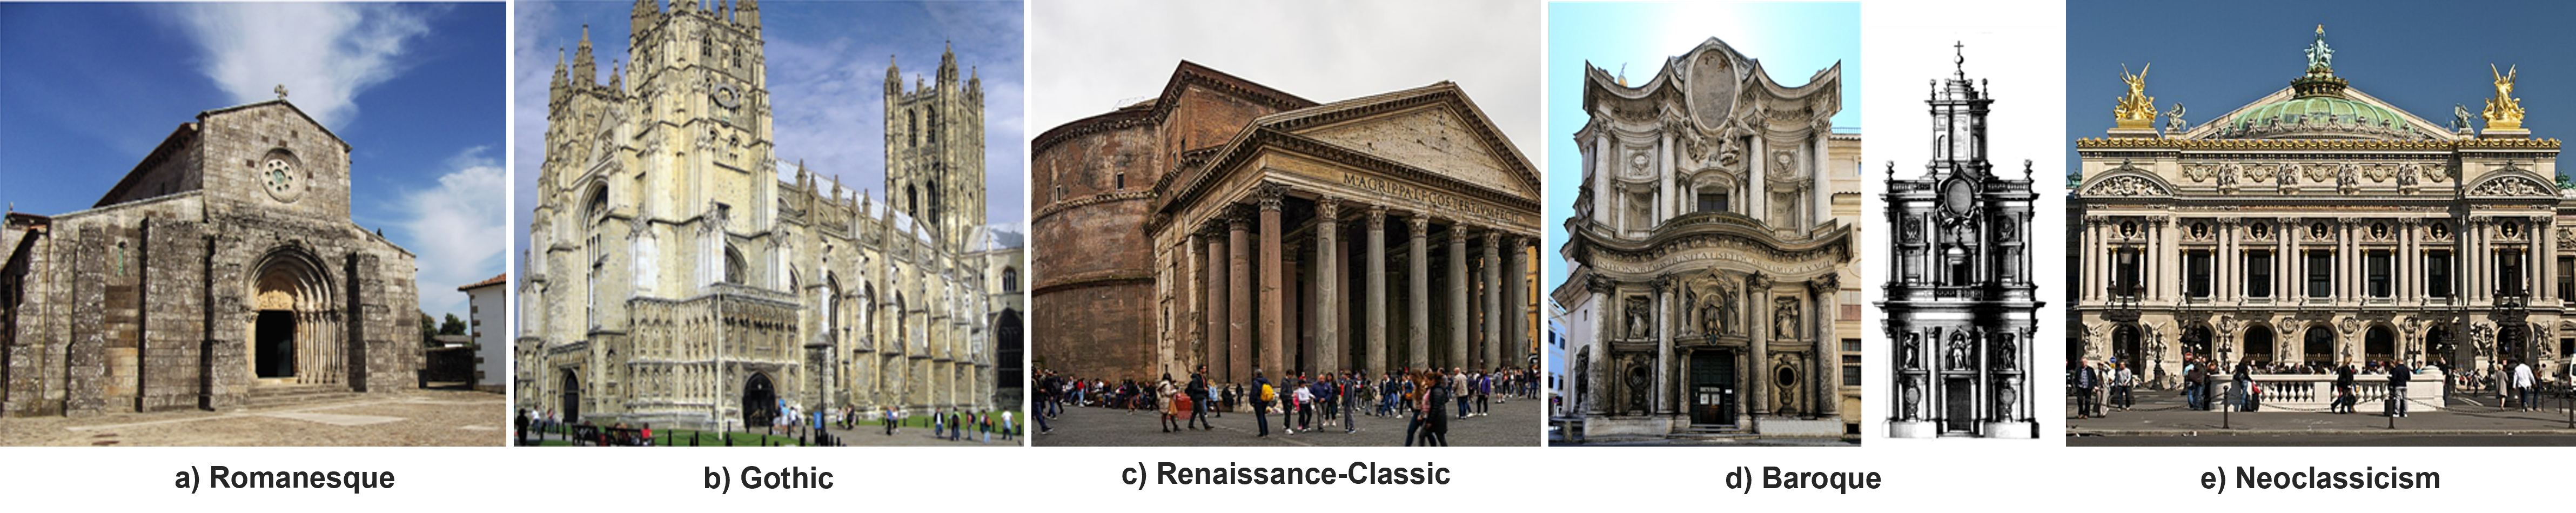
\includegraphics[width= \linewidth]{Images/OldTimeline}
                    \captionof{figure}{Example of historical oscillations between complexity and simplicity in architecture history. (Left to right) Romanesque, Gothic, Classicism, Baroque, Neo-classicism. (\textit{Images edited from source})}
                    \label{fig:Oldtimeline}
                    \\
                    \centering
                    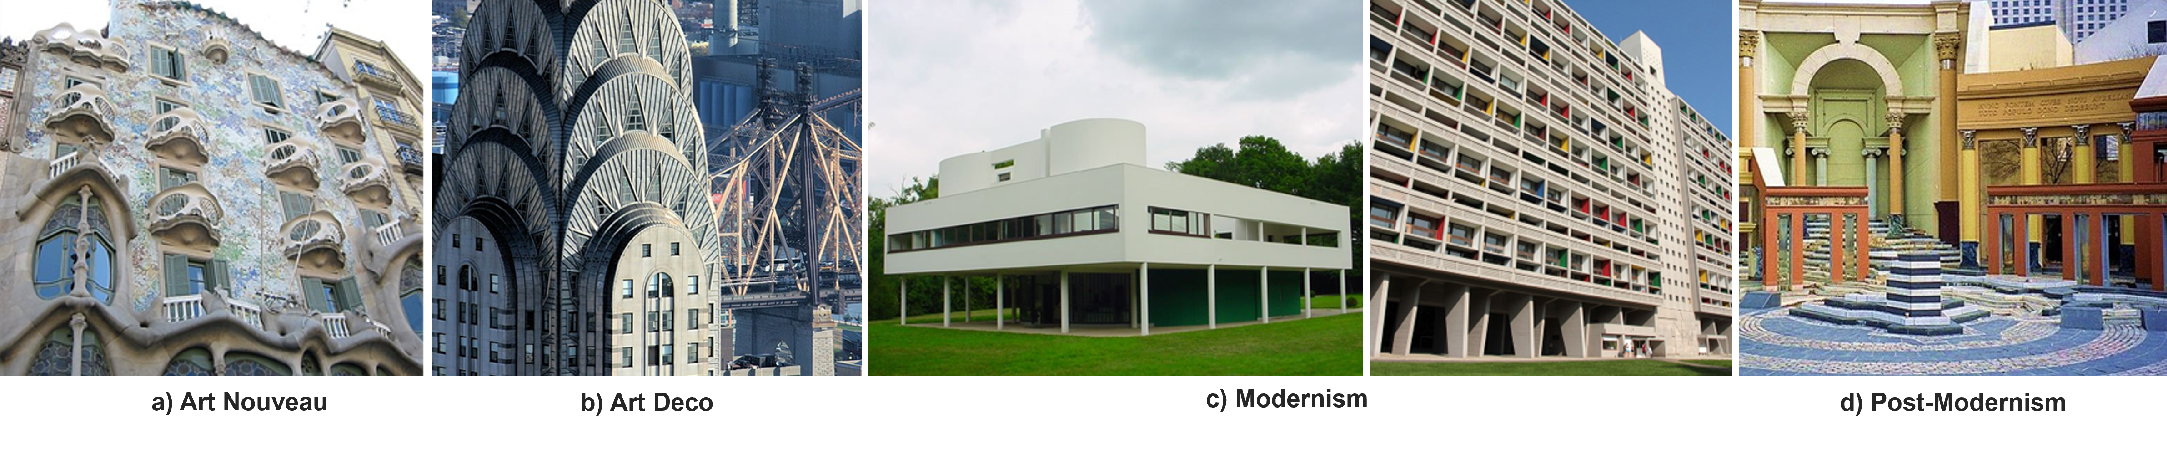
\includegraphics[width= \linewidth]{Images/MiddleTimeline}
                    \captionof{figure}{Example of historical oscillations between complexity and simplicity in architecture history. (Left to right) Art Nouveau, Art Deco, Modernism, Post Modernism. (\textit{Images edited from source})}
                    \label{fig:Middletimeline}
                    \\
                    \centering
                    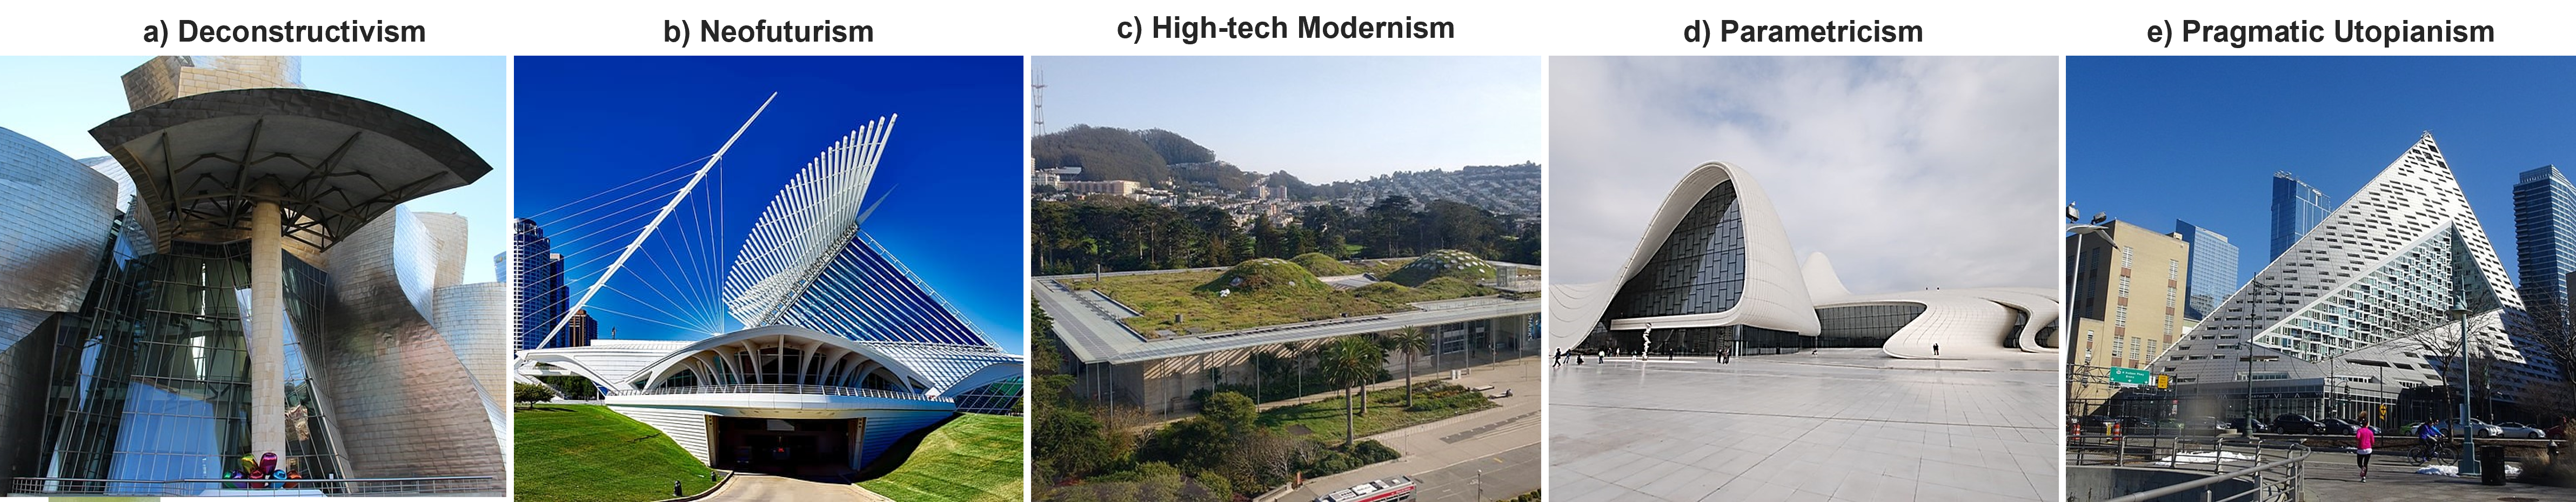
\includegraphics[width= \linewidth]{Images/contemporaryTimeline}
                    \captionof{figure}{Era of exploration in contemporary architecture. (Left to right) Deconstructivism, Neofuturism, High-tech modernism, Parametricism, Pragmatic utopianism. (\textit{Images edited from source})}
                    \label{fig:contemporarytimeline}
                \end{tabularx}
            \end{table*}

\section{Theory Framework}
\label{sec:Theory Framework}
%% Research Background

%% A Theory section should extend, not repeat, the background to the article already dealt with in the Introduction and lay the foundation for further work. In contrast, a Calculation section represents a practical development from a theoretical basis.

%A theoretical framework is a foundational review of existing theories that serves as a roadmap for developing the arguments you will use in your own work.

%=============================================================================
%Outline.
%1. Introduction
%2. The importance of facade in a building.
%3. A brief analysis of architecture styles and the
%3. A reflexion into digital fabrication techniques specially parametric design.
%4. The principle od data driven design.
%5. An analysis into mixed reality and the advantages of introducing this  into the design review.
%=============================================================================

%///////////////////////////////////////////////////////////////
%% refined outline of theory framework

%6. **Human-Centric Design Philosophy:** Explore the historical evolution of architectural philosophies that prioritize human experience and well-being. Discuss how different architectural styles and movements have addressed the balance between ornamentation, functionality, and human comfort.

%7. **Cultural Significance of Facades:** Delve deeper into how facades reflect cultural values, societal norms, and historical contexts. Explore how different societies and civilizations have expressed their identity through architectural ornamentation and symbolism.

%8. **Environmental Sustainability:** Investigate how the integration of complex facades and digital fabrication aligns with contemporary sustainability principles. Examine how parametric design and data-driven approaches can enhance energy efficiency, reduce material waste, and contribute to sustainable construction practices.

%9. **Ethics and Social Responsibility:** Consider the ethical implications of embracing ornate designs and digital fabrication in a world grappling with issues of resource scarcity and inequality. Discuss how responsible architectural practices can address these challenges and contribute positively to society.

%10. **Collaborative Design Process:** Explore the collaborative aspects of architectural design when utilizing digital fabrication and mixed reality. Discuss how these technologies foster interdisciplinary collaboration among architects, engineers, urban planners, and other stakeholders.

%11. **Challenges and Limitations:** Address the potential challenges and limitations of implementing complex facades and digital fabrication techniques. Discuss technical, economic, and cultural barriers that may arise and the strategies to overcome them.

%12. **Case Studies and Success Stories:** Showcase real-world examples of projects that have successfully integrated complex facades, digital fabrication, and mixed reality. Analyze the impact of these projects on user experience, urban aesthetics, and architectural innovation.

%13. **User-Centered Design:** Delve into the principles of user-centered design and human factors that influence the acceptance of intricate facades. Consider factors like psychological comfort, emotional response, and sensory experience in relation to complex architectural designs.

%14. **Cognitive Aspects of Mixed Reality:** Explore the cognitive psychology behind mixed reality experiences and how they influence user perceptions of architectural complexity. Consider how elements like immersion, presence, and interaction affect users' understanding and appreciation of design.

%15. **Future Trends and Speculation:** Speculate on the potential future trajectories of architectural design, digital fabrication, and mixed reality. Discuss how these trends might shape the built environment, and propose ideas for further research and exploration.

%By incorporating these additional topics into your theory framework, you can provide a comprehensive and well-rounded context for your research, offering deeper insights into the historical, cultural, ethical, and technological dimensions of complex facades, digital fabrication, and mixed reality in architecture.
%///////////////////////////////////////////////////////////////

%% Introduction

Architecture, as a reflection of society, has continually evolved to accommodate the needs of the communities it shelters.
Buildings, in essence, serve as tools with a purpose—guardians of societies, nurturers of generations, and manifestations of future aspirations.

Critique is inherent to architecture, and it falls upon successive generations to discern flaws within the inherited built environment.
Amidst these legacies, the legacy of the modernist movement, emerging in the mid-20th century, emerges as particularly relevant.
Anchored in principles of simplicity and the maxim ``form follows function'', this movement gained global prominence, addressing urbanization challenges triggered by rural migration to cities.

Yet, this era's legacy brings forth a profound debate.
While remarkable creations emerged, it's important not to label nearly a century of architectural style as universally negative.
However, society acknowledges the unintended consequences.
The fervor for uniformity and minimalism, epitomized by modernism, led to a disconnect from cultural roots.
As cities embraced this discourse, they lost distinct identities, homogenizing urban landscapes and erasing their unique memories.

This realization underscores the complex narrative of architecture—a dynamic interplay between innovation, utility, and cultural heritage.
It reminds us that while architectural styles may have their merits, the preservation of cultural essence and identity is vital for thriving urban spaces that resonate with inhabitants and stand the test of time.

 Because as Gage~\cite{Gage2015} eloquently puts it ``If architecture is to exist in the 21st century, when attention is focused on the fast-paced worlds of technology, fashion, and entertainment, it must not recede into the background as mere functional equipment''.

As we delve into the theory framework that underpins this research, we embark on a journey through historical shifts between architectural complexity and simplicity.
We explore the significance of facades in shaping the identity of structures.
We reflect on the integration of digital fabrication techniques, particularly parametric design, and the fundamental principles of data-driven design.
Our exploration extends to the realm of mixed reality and the promising advantages it introduces to the architectural design review process.

Each component within this theory framework contributes to our understanding of the intricate interplay between architectural evolution and societal dynamics.
As we navigate through complexities and contemplate the subtleties of design paradigms, we seek to uncover insights that illuminate the path to a more harmonious relationship between built environments and the people who inhabit them.

\subsection{Human-Centric Design Philosophy across the history of architecture styles}
\label{subsec:TimelineArchitectureStyles}

%%Human-Centric Design Philosophy: Explore the historical evolution of architectural philosophies that prioritize human experience and well-being. Discuss how different architectural styles and movements have addressed the balance between ornamentation, functionality, and human comfort.


Architecture stands as a unique art form, setting itself apart from other creative mediums.
It requires not only the transformation of the ordinary into the extraordinary, akin to painting and sculpture, but also the imperative to fulfill the purpose and functionality of a building\cite{Hnin2022}.

At the core of architectural evolution resides a dynamic interplay between simplicity and complexity, often guided by the intersection of societal values and technological advancements\cite{Economakis2023}.
However, it's important to clarify that within the context of this research, neither simplicity nor complexity carry any inherent negative or positive connotations.
Using the term ``simplicity`` here doesn't imply a condemnation of one style in favor of another;
rather, it highlights that throughout the history of architecture and its various styles, there have been periods characterized by evident complexities as well as phases where designs embraced apparent simplicities that hid their intricacies into themselves.
Undoubtedly, every prevailing architectural style of its time has contributed masterpieces to the built environment.

Consider, for instance, the transition from the robust Romanesque classic style of the 10th century, notably exhibited in churches, to the Gothic style brought by groundbreaking advancements of the 12th century that introduced buttresses, revolutionizing load distribution\cite{Arora2023}(see Figure\ref{fig:RomanesquevsGothic}).
This innovation propelled churches skyward, inviting luminous interplays to embellish the interiors through stunning stained-glass windows bedecked in intricate design\cite{Stacbond2020}.

This trend resurfaced as time unfolded, transitioning from the complex Gothic style to the revival of Greek and Roman ideals, exemplified by the symmetrical perfection of the Renaissance era in the 14th century.
This resurgence was succeeded by the opulent ornamentation of the Baroque style in the 16th century, followed by the neoclassical revival of the 18th century, heavily influenced by classical Greek and Palladian architecture.

In the 1920s and 30s, the intricate Art Deco movement emerged, celebrating technological progress through luxurious materials and patterns seamlessly integrated with modern design and manufacturing techniques.
In response to this progression, the first half of the 20th century witnessed the emergence of Modern Architecture and rationalism.

This architectural ethos adopted the maxim ``Form follows function'', emphasizing functionalism and characterized by a rejection of traditional ornament in favor of new forms of more subtles intricacies like the “aesthetics of machinery” that showcased architecture  enriched  with  only  the  beauty of its lines and the use of new-age materials such as steel, glass, and concrete\cite{Gage2015}(see Figure\ref{fig:ArtDecovsModernism}).
The postmodernism style of the late 60's marks a radical return of ornament in form recognizing that even simplified modern elements serve as ornamentation focusing on the thought of freeing design element from oppresive modern constraints.
The  beginning  of  the  1980s marked a shift towards more imaginative and expressive architecture following architects like Frank Gehry, Zaha Hadid and Rem koolhaas who treated their constructions as monuments of Ornament that transformed architecture into a media.
With highly complex shapes brought into reality by the incorporation of digital technologies.
Examples abound in this era ranging form justaposition of complex ornaments over simple facades to the transformation of ornament not as an articulate material, but as a form of structure, turning the structure to building and ornament.
However due to the complex fabrication that such examples require and expertise, they are not a part of the urban fabric but rather sporadic cases across the globe which can truly be considered as the defining contemporary style, however the democratization of digital fabrication could bring the tools require to create said structures around the world diversifying among cultures and providing authentic interpretations of their context express in the form of complex buildings. This is the time of complexity and ornament.

``If architecture is to exist in the 21st century, when attention is focused on the fast-paced worlds of technology, fashion, and entertainment, it must not recede into the background as mere functional equipment''\cite{Gage2015}.


\subsection{Cultural Significance of Facades and Ornament}
\label{subsec: FacadeandOrnament }
The resonance of Louis Sullivan's renowned phrase, ``Form follows function,`` throughout the Modernist movement of the 20th century and its continued influence on subsequent decades can be attributed to the pivotal role of a building's purpose and functions as the genesis and core of a project\cite{Hnin2022}.

This principle found its radicalization within the context of the times, partly due to a prevailing stance against ornamentation, often dismissed on moralistic grounds.
This sentiment deemed everything beyond function as secondary, exemplified by works like Adolf Loos' 1908 article ``Ornament and Crime,`` which advocated for functional design by condemning traditional ornamentation as superfluous\cite{Saglam2014}.

Even during this era when ornamentation was viewed unfavorably, prominent figures of the time, such as Le Corbusier, who publicly championed the functional ideology, would ingeniously devise methods to infuse their creations with a distinct form of ornamentation, albeit one rooted in materials' textures, structural elements, and inventive ways of articulating functionality.\cite{Saglam2014}.
In Venturi's opinion\cite{Venturi1972} 1960's ``Modern architecture uses expressive ornament and shuns explicit symbolic  ornament'' and all the simplistic facades are a type of ornament\cite{Saglam2014}.

          ``If architecture is to exist in the 21st century, when attention is focused on the fast-paced worlds of technology, fashion, and entertainment, it must not recede into the background as mere functional equipment''\cite{Gage2015}.

          According to Krier the mature city achieves balance with nature and with the people that it serves in its scale, size and integration of residential, commercial and civic functions.
          Krier argues that the reconstruction of a city is a moral imperative, a global project that it is at once cultural social economic and ecological. Time of video 1:06:29

We evidence this when observing the Romanesque classical style on the 10 th century found mostly in churches ith thick wall structures, followed by the breakthrough in load distribution during the Gothic style of the 12th to the 16th century which abandons the robustness to erect high buildings with complex great stained windows.
The Renaissance follows at the end of the Middle Ages and with it the return of the classical order with round arch and classical order columns that brings ornaments back to the interior in favour of more simplified exteriors.
In reaction to this style Baroque style surges with more dynamic forms , irregular shapes and exaggerated ornamentation in bold combinations.

%%%%
what initially motivates this research is the conscious realization that
Upon delving into the annals of influential architectural styles, a discernible pattern emerges—an oscillation between simplicity and complexity(see Figure\ref{fig:TimelineArchitecture}).
This recurrent cycle in architectural paradigms is not only reflective of the values ingrained in the societies they house, but also closely tied to pivotal technological advancements.
Consider, for instance, the transition from the Romanesque style of the 10th century to the Complex Gothic style 12th style, replaced by the revival of greek and roman ideals during the Renaissence style, followed by the complex opulent ornamentation of the Baroque style in the 16th century replaced by the neoclassical revival of the 18th century, heavily influenced by classical Greek and Palladian architecture\cite{Arora2023}.
This pattern repeats all the way to the 1920s and 30s, the intricate Art Deco will be replaced on the first half of the 20th century witnessed the emergence of Modern Architecture and rationalism emphasizing functionalism and minimalistic architecture




This shift encapsulates the quintessence of architectural evolution—an ever-changing interplay between simplicity and complexity, often steered by the confluence of societal values and technological breakthroughs.


Once again, we find ourselves at a pivotal juncture in history, as the emergence of computer-aided design converges with the industrialization of construction, ushering in a new paradigm in architectural design.
The 20th-century dominance of Rationalism, exemplified by figures like Le Corbusier, underscored an ethos of oversimplification and functionality.
Characterized by straightforward, symmetrical forms and concrete as the favored medium, this era yielded cities estranged from human-centric design.
Swift transportation took precedence, fracturing urban spaces that once defined vibrant societies\cite{Stacbond2020}.
Subsequently, industrial design asserted its dominance as the blueprint for future construction\cite{Economakis2023}, casting architecture in the mold of minimalism and mass-produced uniformity, forsaking the ornate allure and individuality of yesteryears.

\subsection{Object-Oriented Ontology}
\label{subsec:ObjectOrientedOntology}
% add the concept of Object-Oriented. Using these concepts as basis. I want to express that the mr experiment is based on the idea that architecture as a tool should be invisible and confortable while in use. But it should  create emotion when seen as part of the landscape as a form of art to recapture the humand oriented city .

Heideggers tool analysis states that as the tool is a tool it disappears in favor of some purpose he continues to explain that generally we don't notice equipment until it fails, like when An earthquake calls attention to the ground we walk or when a medical problem alerts us of the presence of organs that we have silently depended\cite{Harman2011}.
Harmans, Object-oriented ontology, borrows this concept to formulate its central claim that objects have hidden qualities and realities, and they withdraw from our understanding.\cite{Gage2015}
he idea that we live our lives on a layer of invisible equipment has significant ramifications for architecture, a discipline that produces the equipment on and in which we exist.\cite{Gage2015}


    \subsection{Human-Centric Design Philosophy across the history of architecture styles}
    \label{subsec:TimelineArchitectureStyles}
    \input{Text/TheoryHistoryArchStyles}

    \subsection{Cultural Significance of Facades and Ornament}
    \label{subsec:FacadeandOrnament}
    
%!subsection{Cultural Significance of Facades and Ornament}
%!\label{subsec: FacadeandOrnament}

%!==========================
%Delve deeper into how facades reflect cultural values, societal norms, and historical contexts. Explore how different societies and civilizations have expressed their identity through architectural ornamentation and symbolism.
%!==========================

%!Concise version
Architecture, transcending its primary role of providing shelter, serves as a canvas reflecting the cultural, historical, and societal narratives of its time.
Facades and ornamentation, in this context, become critical in conveying these narratives, bridging the gap between the aesthetic and the symbolic, and establishing the interface between buildings and their environments, influencing comfort and energy efficiency, while reflecting the building's identity\cite{Kamal2020}.

While the previous section traced the oscillations between simplicity and complexity in architectural styles to establish a foundation for the notion that contemporary architecture is gravitating towards a renaissance of complexity, here we explore the underlying cultural currents that influenced these shifts.
The evolution of facade design and ornamentation mirrors societal transformations, technological progress, and shifts in artistic sensibilities, each impacting how communities relate to their built environment.

%Facades according to Vitruvius

Vitruvius, in his 1st-century BCE work `De Architectura', outlined principles for architecture that emphasize structural soundness, functionality, and beauty\cite{Ostwald2023}.
He advocated for harmony and balance in design, using the principle of `Decor' to guide appropriate articulation that respects religious, natural, and social conventions\cite{Lefas2000}.
Vitruvius's principles, dormant for centuries, found renewed interest during the Renaissance and continued through the Neoclassical and Ecole des Beaux-Arts styles\cite{Wikipedia2023}.
This revival reinforced the classical architectural aesthetics rooted in order and rationality (Figure\ref{fig:Oldtimeline} c,e).
The principles of Vitruvius, emphasizing a balance of structural integrity, functionality, and aesthetics, have had a lasting impact, shaping the trajectory of architectural design and ornamentation throughout history.

%facade according to bernini and borromini

Moving beyond the Renaissance era and into the Baroque style, a significant shift in the perception of facades and ornamentation occurs.
Francesco Borromini, a prominent Italian architect of the Baroque period, emerges as a key figure in this context.
Borromini's architectural philosophy revolved around the facade as a reflection of a building's interior.
He viewed the facade not just as an ornamental feature but as a visual representation of the internal spaces and functions\cite{Benjamin2006}.
Borromini's designs often featured elaborate geometric patterns, curved forms, and sculptural elements, integrating the facade with the building's spatial organization and internal arrangement.
This approach is exemplified in his works, such as the San Carlo alle Quattro Fontane Church in Rome (Figure\ref{fig:Oldtimeline} d).

Borromini's perspective on facades transcended surface aesthetics.
He believed facades should express the building's deeper design and purpose, embodying an expressive display of interiority and an invitation for an external reading\cite{Biglieri2004}.
This philosophy underscores the integral role of facades in the overall architectural composition during the Baroque period.

% context on neo classic, art nouveau and art deco

In tracing the evolution of facades and ornamentation, it's important to recognize the architectural periods that significantly influenced the field, bridging the gap between the Baroque era and the transformative epoch of Modernism.
Notable styles in this transition include Neo-Classicism, Art Nouveau, and Art Deco.

Neo-Classical architecture (late 18th to early 19th centuries) revived Vitruvian principles and Palladian ideals.
It emphasized formal elegance and symmetry, often featuring facades with balanced proportions and columns (Figure\ref{fig:Oldtimeline} e).
Art Nouveau (late 19th to early 20th centuries), led by architects like Gaudi, introduced organic forms into facade design.
Gaudi's work, such as Casa Batlló, utilized flowing lines and natural motifs\cite{Nasir2022} (Figure\ref{fig:Middletimeline} a).
Art Deco (1920s to early 1930s) merged luxury and technological progress, characterized by geometric shapes, high-contrast colors, and metallic surfaces, as seen in the Chrysler Building\cite{Kotb2014} (Figure\ref{fig:Middletimeline} b).
While these styles contributed to the diversity of architectural aesthetics, they did not initiate the profound paradigm shifts that Modernism would later bring.
With this context, we now turn to the significant impact of the Modernist movement on architectural philosophy.

% Modernism and facade according to Le Corbusier

The transition into the 20th century's Modernist style marked a significant shift in the approach to facades and ornamentation.
As discussed in the previous section, this era, saw a move away from traditional ornamental design.

Loos, in his 1908 article `Ornament and Crime', a prominent figure on this movement, championed functional design and critiqued conventional ornamentation\cite{Saglam2014}.
Le Corbusier, a key Modernist architect, further revolutionized facade design.
His work, particularly `Towards a New Architecture'\cite{Studio2a2023} and `The Five Points of a New Architecture', emphasized minimalism and utility.
He advocated for facades that reflect a building's purpose and the well-being of its occupants, adhering to his human-centric design philosophy\cite{Virseda2021}.

Le Corbusier's concept of `Free design of the facade'\cite{Corbusier1986} allowed for innovative use of materials and structural elements to create functional ornamentation.
His designs often featured large windows, sunshades, and brise-soleil, prioritizing light, ventilation, and climate control while maintaining aesthetic integrity (Figure\ref{fig:Middletimeline} c).
Thus, Le Corbusier's views on facades represent a blend of clarity, rationality, and harmonious integration, rejecting excess adornment while celebrating structural innovation and technological advancements.

% Postmodernism and facade according to Venturi

Despite the innovative drive of Modernism, its utopian vision often fell short in materializing human-centric environments, leading to spaces that felt monotonous and detached from cultural contexts.
This paved the way for Robert Venturi's critical perspective on Modernism and his pioneering role in the Postmodernism movement.

Venturi, in his seminal works like `Complexity and Contradiction in Architecture' and `Learning From Las Vegas', challenged the Modernist ideals, advocating for architecture that embraced complexity, contradiction, and meaningful ornamentation \cite{Venturi1977}.
He criticized the Modernist approach for its oversimplification and lack of symbolic expression, arguing for an architecture that responds to cultural context and human experience (Figure\ref{fig:Middletimeline} d).



Venturi's approach to facades and ornamentation incorporated diverse elements, historical references, and bright colors, challenging the minimalist ethos of Modernism.
He believed in the richness of symbolism and the importance of integrating elements from historical precedents into contemporary design\cite{Venturi1971}.
His famous dictum, `Less is a bore', encapsulated his critique of Modernist minimalism and his advocacy for thoughtful ornamentation.

Venturi's vision encouraged the use of facades as mediums to communicate various meanings, evoke emotions, and respond to their cultural and contextual surroundings.
His influence in Postmodernism expanded architectural horizons, urging architects to embrace diversity, historical resonance, and meaningful expression in their designs\cite{Lutolli2020, Stamp2016}

%Contemporary styles

Following Postmodernism, contemporary architecture witnessed a shift towards more dynamic and diverse styles, including Deconstructivism, Neofuturism, High-tech modernism, Parametricism, and Pragmatic utopianism.
These styles collectively signify a move towards complexity in facade design and ornamentation, influenced by advancements in technology and a focus on sustainability.

Deconstructivism, characterized by fragmentation and non-rectilinear shapes, was exemplified by architects like Frank Gehry, who integrated unconventional forms into their designs (Figure\ref{fig:contemporarytimeline} \textit{a}).
Neofuturism, represented by architects like Santiago Calatrava, embraced a futuristic aesthetic with dynamic, flowing forms (Figure\ref{fig:contemporarytimeline} \textit{b}).
High-tech modernism, or structural expressionism, focused on showcasing technological components and advanced materials, as seen in works by Renzo Piano and Norman Foster (Figure\ref{fig:contemporarytimeline} \textit{c}).
Parametricism, often associated with Zaha Hadid, utilized computational design to create intricate geometries and dynamic structures (Figure\ref{fig:contemporarytimeline} \textit{d}).
Pragmatic utopianism, exemplified by Bjarke Ingels, combined ambitious visions with practical solutions, focusing on functionality, sustainability, and meaningful ornamentation (Figure\ref{fig:contemporarytimeline} \textit{e}).
These styles reflect the architectural evolution from the late 20th century into the 21st, showcasing a variety of approaches to facades and ornamentation that blend tradition with innovation.


%conclusion
In conclusion, the journey through the evolution of facade and ornament theory reveals a rich tapestry of architectural ingenuity, shaped by cultural, technological, and artistic influences.
From the foundational principles of Vitruvius to the ornate expressions of the Baroque period, the functional minimalism of Modernism, and the eclectic approaches of Postmodernism, each era has contributed distinct perspectives on the relationship between a building's exterior and its intrinsic character.

Contemporary styles like Deconstructivism, Neofuturism, High-tech Modernism, Parametricism, and Pragmatic Utopianism (see Figure\ref{fig:contemporarytimeline}) further demonstrate the diversity and dynamism in current architectural practice.
These styles collectively underscore an ongoing dialogue between simplicity and complexity, tradition and innovation, functionality and aesthetics.

As we look towards the future, the continued evolution of facade and ornament theory will undoubtedly be influenced by emerging technologies, sustainability concerns, and the ever-changing needs of human societies, shaping the built environment in ways that are both imaginative and responsive to the world around us.

The cultural significance of facades extends beyond aesthetic appeal, contributing to a community's sense of identity and continuity.
As we look to the future, the challenge and opportunity lie in harnessing emerging technologies to create architecture that resonates with societal values and cultural diversity, thereby enriching the urban landscape.






    %\subsection{Digital fabrication and Environmental Sustainability}
    %\label{subsec:DigitalFabricationAndEnvSustainability}
    %
%!\subsection{Digital fabrication and Environmental Sustainability}
%!\label{subsec:DigitalFabricationAndEnvSustainability}

%!==========================
%8. **Environmental Sustainability:** Investigate how the integration of complex facades and digital fabrication aligns with contemporary sustainability principles. Examine how parametric design and data-driven approaches can enhance energy efficiency, reduce material waste, and contribute to sustainable construction practices.
%!==========================
To be revised ...
%!original

%Digital fabrication technologies, meanwhile, are interacting with the biological world on a daily basis.
%Engineers, designers, and architects are combining computational design, additive manufacturing, materials engineering, and synthetic biology to pioneer a symbiosis between microorganisms, our bodies, the products we consume, and even the buildings we inhabit\cite{Schwab2016}.







            %!% Figures Methodology intro
            %% Methodology Flowchart
            \begin{figure*}[!htb]
                \centering
                \includegraphics[width= \linewidth]{Images/MethodologyFlowchart}~\caption{Methodology Flowchart illustrating the sequential steps of this study's approach framework designed to assess the tolerance of users towards complex facade design. Higlighting the transition from VR system development (\ref{subsec:VRsystemDevelopment}), experiment design (\ref{subsec:Experiment_design}) and post-experiment data analysis phase. }
                  \label{fig:MethodologyFlowchart}
            \end{figure*}

\section{Methodology}
\label{sec:Methodology}
%%Methodology
%% methodology Intro
The methodology of this study, comprises three main components (as illustrated in  Figure~\ref{fig:MethodologyFlowchart}):

\begin{itemize}
    \item Computational Image Complexity Analysis (CICA) system
    \item VR System Development
    \item Experiment Design
\end{itemize}

\textbf{CICA system:} Detailed in Section~\ref{subsec:Computational Image Complexity analysis} and depicted as (3.1) in Figure~\ref{fig:MethodologyFlowchart}, involves developing a Python script using computer vision algorithms to process images and yield complexity scores, quantitatively gauging the intricacy of architectural designs.
It supports theoretical analyses and provides a ranking framework for facade designs in the VR system.

\textbf{VR System Development:}  Outlined in Section~\ref{subsec:VRsystemDevelopment} and represented as (3.2) in Figure~\ref{fig:MethodologyFlowchart}, this component focuses on creating an immersive experience where participants can explore and interact with a building's interior and exterior, manipulating facade designs with variable complexity levels and experiencing their impact.

\textbf{Experiment Design:} Detailed in Section~\ref{subsec:Experiment_design} and illustrated as (3.3) in Figure~\ref{fig:MethodologyFlowchart}, following a similar approach to previous studies~\cite{Wolfartsberger2019}, this component outlines the method to evaluate users' acceptance of building complexity.
It consists of three stages: a VR interaction stage, a screen-based stage, and a post-interaction survey.
These stages allow for the collection of quantitative and qualitative data on participants' perceptions and responses to different complexity levels in facade designs.

As illustrated in the methodology flowchart (Figure~\ref{fig:MethodologyFlowchart}), these components are combined to integrate computational analysis with immersive VR experiments, exploring user preferences in facade design and providing insights into architectural trends.

With this methodology outlined, the following sections will now delve into a comprehensive breakdown of each component, highlighting their objectives, methodologies, and significance in achieving our research goals.




            %!%Figures and table CICA
            %Flowchart CICA, Figure of Cica on historical buildings and renders, PI table. Table 1x3
            \begin{table*}[h!tb]
                \centering
                \small
                \begin{tabular}{c}
                    %Top cell with one figure
                    %Figure Computational Image Compexity Analysis (CICA) System flowchart
                    \begin{minipage}{\textwidth}
                        \centering
                        \includegraphics[width= \linewidth]{Images/ImageComplexityAnalysisFlowchart}
                        \caption{Flowchart illustrating the applications of Computational Image Complexity Analysis, including its role in analyzing complexity scores for historical architectural styles and ranking modeled facades for the VR Building Complexity System.}
                      \label{fig:ImageComplexityAnalysisFlowchart}
                    \end{minipage}
                    \\
                    %Middle cell with two nested figures side by side
                    %%%Figure CICA on historic buildings and renders. Table 1x2
                    \begin{minipage}{\textwidth}
                        \centering
                        % Left figure
                        \begin{minipage}{0.49\textwidth}
                            \includegraphics[width= \linewidth]{Images/ComplexityPlotHistoryCICA}
                            \captionof{figure}{Edge Detection analysis of historic buildings demonstrating complexity assessment.}
                            \label{fig:ComplexityPlotHistory}
                        \end{minipage}
                        \hfill % Spacing between the figures
                        % Right figure
                        \begin{minipage}{0.49\textwidth}
                            \includegraphics[width= \linewidth]{Images/ComplexitPlotRenderCICA}
                            \captionof{figure}{Complexity analysis of 3D-modeled facades for the VR experiment.}
                            \label{fig:ComplexityPlotRenderCICA}
                        \end{minipage}
                    \end{minipage}
                    \\
                    %Bottom cell
                    %Table: Performance Indicators
                    \begin{minipage}{\textwidth}
                        \centering
                        \captionof{table}{Metrics and weights for the calculation of the `Complexity score'}
                        \label{tab:MetricsandWeights}
                        \begin{tabularx}{\textwidth}{p{3.5cm} p{1cm} X X p{1cm}}
                            \toprule
                            \textit{Complexity metric} &
                              \textit{N} &
                              \textit{Metric name/description} &
                              \textit{Quantitative   method} &
                              \textit{Weights} \\ \midrule
                            \textbf{Edge Density} &
                              1 &
                              Edge detection using Canny Edge Detection algorithm for highlighting the most relevant features of a building.
                                &
                              Measured by dividing the number of non-zero (edge) pixels in the edges image by the total number of pixels in the image.
                                &
                              8\\
                            \textbf{Contour count} &
                              2 &
                              Employs contour approximation algorithm for shape analysis to determine intricacy of edges.
                                &
                              Measure by counting the number of segments in an edge.
                                &
                              2\\ \bottomrule
                               &
                               &
                              \textbf{TOTAL} &
                              &
                              \textbf{10}\\ \bottomrule
                        \end{tabularx}
                    \end{minipage}
                \end{tabular}
            \end{table*}

            %f1: Complexity scoring function
            \begin{table}[htb]
                \caption{Complexity scoring function }
                \label{tab:ComplexityScoreFunction_table}
                \centering
                \small
                \begin{tabular}{|p{8cm}|}
                \hline
                    \textbf{\(f_1\), Unified `Complexity Scoring' function 1}\\
                    \textit{Calculate the complexity score for all the images on the data pool}
                    \\
                    \begin{equation}
                        f_1(x) = \left[ \mathrm{round}\left(\sum_{i=1}^{n} w_i \cdot a_i, 2\right) \right] = complexity\_score
                    \label{eq:F1_ComplexityScoreFunction}
                    \end{equation}

                    \\
                    \textit{ for the Buildings included in the database.}\\
                    \\
                    \textit{where;} \\
                    \\
                    \(n \); is the number of performance indicators \\
                    \(w_i \); represents the i-th elements weight input and \\
                    \(a_i \); represents the i-th normalized score for the respective metric(`Edge Density' and `Contour Count').\\
                    \\

                    \textit{Finally, the `Complexity score' is assigned to each building for data visualization.}\\
                \hline
                \end{tabular}
            \end{table}

            %% Figure of Complexity graph
            \begin{figure*}[!htb]
                  \centering
                  \includegraphics[width= \linewidth]{Graphs/complexitygraphrender}
                  \caption{Scatter graph showcasing quantitative Computational Image Complexity Analysis scores for the rendering images of the 10 variations for each of the three patterns modeled in Blender, with an overlaid trendline highlighting the complexity level trend towards increased complexity.}
                  \label{fig:complexitygraphRender}
            \end{figure*}


    \subsection{Computational Image Complexity Analysis (CICA) system}
    \label{subsec:Image Complexity analysis}
    % this section describes the computational image complexity analysis
%!Concise version
The theory framework section meticulously examined the architectural evolution, revealing a recurring cycle oscillating between complex and simple styles.
Given the recent technological advancements and contemporary architectural trends, there is a compelling indication that the present era is poised for a shift toward complexity, countering the preceding Modernist movement characterized by minimalism and simplicity.

In pursuit of validating this hypothesis, we developed a Computational Image Complexity Analysis (CICA) system.
Our primary objective was to not only empirically validate the trends in architectural complexity suggested by our theoretical analysis but also to create a quantifiable metric.
This metric would play a crucial role in evaluating and ranking the 3D-modeled facades intended for use in the Virtual Reality experience.

The Computational Image Complexity  Analysis (CICA) system is a Python function that assesses complexity by quantifying the number of elements within a building's design and analyzing their shapes.
The higher the count of elements, the higher the assigned complexity score, and vice versa.
This approach draws inspiration from Venturi et al.'s reflection on complexity, as articulated in their work\cite{Venturi1977}.
They posited that a building's complexity could be gauged by the time it takes to mentally process and form a coherent image of its constituent elements.
This fundamental concept underpins the CICA system's methodology(Figure\ref{fig:ImageComplexityAnalysisFlowchart}).

%% Figure Computational Image Compexity Analysis (CICA) System flowchart
    \begin{figure}[!htb]
      \centering
      % trim=left 190 down 250 right 150 top5
      \includegraphics[width= \linewidth, trim=0 0 0 0, clip]{Images/ImageComplexityAnalysisFlowchart}
      \caption{Flowchart illustrating the applications of Computational Image Complexity Analysis, including its role in analyzing complexity scores for historical architectural styles and ranking modeled facades for the VR Building Complexity System.}
      \label{fig:ImageComplexityAnalysisFlowchart}
    \end{figure}

The CICA system evaluates complexity through two metrics: edge density, using the Canny Edge Detection algorithm\cite{EdgeOpenCV2023}, and contour count, based on contour approximation\cite{ContourOpenCV2023}.
These metrics are normalized and combined into a unified complexity score (Table\ref{tab:MetricsandWeights}).

    %%Table: Performance Indicators
    \begin{table*}[htb]
        \centering
        \small
        \caption{Metrics and weights for the calculation of the `Complexity score'}
        \label{tab:MetricsandWeights}
        \begin{tabularx}{\textwidth}{p{3.5cm} p{1cm} X X p{1cm}}
            \toprule
            \textit{Complexity metric} &
              \textit{N} &
              \textit{Metric name/description} &
              \textit{Quantitative   method} &
              \textit{Weights} \\ \midrule
            \textbf{Edge Density} &
              1 &
              Edge detection using Canny Edge Detection algorithm for highlighting the most relevant features of a building.
                &
              Measured by dividing the number of non-zero (edge) pixels in the edges image by the total number of pixels in the image.
                &
              8\\
            \textbf{Contour count} &
              2 &
              Employs contour approximation algorithm for shape analysis to determine intricacy of edges.
                &
              Measure by counting the number of segments in an edge.
                &
              2\\ \bottomrule
               &
               &
              \textbf{TOTAL} &
              &
              \textbf{10}\\ \bottomrule
        \end{tabularx}
    \end{table*}

The complexity scoring function \(f_1(x)\) is a crucial part of our CICA system, where the weighted sum of the normalized scores for each metric is calculated, providing an overall complexity score for each building image (Table\ref{tab:ComplexityScoreFunction_table}).

    %f1: Complexity scoring function
    \begin{table}[htb]
        \caption{Complexity scoring function }
        \label{tab:ComplexityScoreFunction_table}
        \centering
        \small
        \begin{tabular}{|p{8cm}|}
        \hline
            \textbf{\(f_1\), Unified `Complexity Scoring' function 1}\\
            \textit{Calculate the complexity score for all the images on the data pool}
            \\
            \begin{equation}
                f_1(x) = \left[ \mathrm{round}\left(\sum_{i=1}^{n} w_i \cdot a_i, 2\right) \right] = complexity\_score
            \label{eq:F1_ComplexityScoreFunction}
            \end{equation}

            \\
            \textit{ for the Buildings included in the database.}\\
            \\
            \textit{where;} \\
            \\
            \(n \); is the number of performance indicators \\
            \(w_i \); represents the i-th elements weight input and \\
            \(a_i \); represents the i-th normalized score for the respective metric(`Edge Density' and `Contour Count').\\
            \\

            \textit{Finally, the `Complexity score' is assigned to each building for data visualization.}\\
        \hline
        \end{tabular}
    \end{table}

In summary, the CICA system leverages two key metrics, edge density and contour count, to quantify the complexity of building facades.
While edge density emphasizes the presence and density of edges, contour count delves into the intricacies of the shapes represented by these edges.
The combination of these metrics provides a more comprehensive and nuanced assessment of architectural complexity, making them valuable tools in our analysis.
Having outlined the development and purpose of the Computational Image Complexity Analysis (CICA) system, we will now delve into its application.

The CICA system's first application is the historical analysis of 180 buildings from various architectural eras (Figure \ref{fig:ComplexityPlotHistory}), resulting in a scatter graph demonstrating complexity trends over time.

The second application involves ranking 3D-modeled facades for the VR experiment.
Using Blender, we modeled facades with varying complexity, categorized into ten levels based on CICA scores (Figure\ref{fig:ComplexityPlotRenderCICA}).
Through CICA, we aim to empirically validate architectural complexity trends and effectively prepare for the VR experiment that assesses user perceptions of facade complexity.
This dual application of the CICA system allows us to quantitatively explore architectural complexity, aligning with our theoretical analysis and providing a basis for further experimentation in VR

%%Figure Canny Edge of historic buildings and renders

\begin{table*}[htb]
    \centering
    \small
    \begin{tabularx}{\textwidth}{X X}
        \centering
        \includegraphics[width= \linewidth]{Images/ComplexityPlotHistoryCICA}
        \captionof{figure}{Edge Detection analysis of historic buildings demonstrating complexity assessment.}
        \label{fig:ComplexityPlotHistory} &
        \centering
        \includegraphics[width= \linewidth]{Images/ComplexitPlotRenderCICA}
        \captionof{figure}{Complexity analysis of 3D-modeled facades for the VR experiment.}
        \label{fig:ComplexityPlotRenderCICA}
        \end{tabularx}
    \end{table*}


%!Original text
%The theory framework section meticulously examined the architectural evolution, revealing a recurring cycle oscillating between complex and simple styles.
%Given the recent technological advancements and contemporary architectural trends, there is a compelling indication that the present era is poised for a shift toward complexity, countering the preceding Modernist movement characterized by minimalism and simplicity.
%
%In pursuit of validating this hypothesis, we developed a Computational Image Complexity Analysis (CICA) system.
%Our primary objective was to not only empirically validate the trends in architectural complexity suggested by our theoretical analysis but also to create a quantifiable metric.
%This metric would play a crucial role in evaluating and ranking the 3D-modeled facades intended for use in the Virtual Reality experience.
%
%The Computational Image Complexity  Analysis (CICA) system is a Python function that assesses complexity by quantifying the number of elements within a building's design and analyzing their shapes.
%The higher the count of elements, the higher the assigned complexity score, and vice versa.
%This approach draws inspiration from Venturi et al.'s reflection on complexity, as articulated in their work\cite{Venturi1977}.
%They posited that a building's complexity could be gauged by the time it takes to mentally process and form a coherent image of its constituent elements.
%This fundamental concept underpins the CICA system's methodology(Figure\ref{fig:ImageComplexityAnalysisFlowchart}).
%
%%% Figure Computational Image Compexity Analysis (CICA) System flowchart
%    \begin{figure}[!htb]
%      \centering
%      % trim=left 190 down 250 right 150 top5
%      \includegraphics[width= \linewidth, trim=0 0 0 0, clip]{Images/ImageComplexityAnalysisFlowchart}
%      \caption{Flowchart illustrating the applications of Computational Image Complexity Analysis, including its role in analyzing complexity scores for historical architectural styles and ranking modeled facades for the VR Building Complexity System.}
%      \label{fig:ImageComplexityAnalysisFlowchart}
%    \end{figure}
%
%The Computational Image Complexity Analysis (CICA) system as shown in Figure\ref{fig:ImageComplexityAnalysisFlowchart} works by using building images as input, subsequently processing these images to enhance contrast and minimize noise, thereby improving the recognition of individual elements within the building's design.
%
%The system employs a method of complexity quantification based on two metrics: edge density and contour count .
%They were chosen by their capabilities in computer vision for identifying edges and shape analysis and whose results are later combined into a unified `complexity score'(see \ref{tab:MetricsandWeights}).
%
%    %%Table: Performance Indicators
%    \begin{table*}[htb]
%        \centering
%        \small
%        \caption{Metrics and weights for the calculation of the `Complexity score'}
%        \label{tab:MetricsandWeights}
%        \begin{tabularx}{\textwidth}{p{3.5cm} p{1cm} X X p{1cm}}
%            \toprule
%            \textit{Complexity metric} &
%              \textit{N} &
%              \textit{Metric name/description} &
%              \textit{Quantitative   method} &
%              \textit{Weights} \\ \midrule
%            \textbf{Edge Density} &
%              1 &
%              Edge detection using Canny Edge Detection algorithm for highlighting the most relevant features of a building.
%                &
%              Measured by dividing the number of non-zero (edge) pixels in the edges image by the total number of pixels in the image.
%                &
%              8\\
%            \textbf{Contour count} &
%              2 &
%              Employs contour approximation algorithm for shape analysis to determine intricacy of edges.
%                &
%              Measure by counting the number of segments in an edge.
%                &
%              2\\ \bottomrule
%               &
%               &
%              \textbf{TOTAL} &
%              &
%              \textbf{10}\\ \bottomrule
%        \end{tabularx}
%    \end{table*}
%
%In the case of edge density, the system utilizes edge detection, to highlight a pronounced edge within an image of a building.
%This can be associated with a distinct element of the building, and in the case of more intricate structures, this script interprets such edges as separations denoting additional architectural elements.
%
%Edge detection is a critical step in our Computational Image Complexity Analysis (CICA) system, performed using the Canny Edge Detection algorithm\cite{EdgeOpenCV2023}.
%This algorithm, readily accessible in Python through OpenCV (cv2.Canny function), is designed for computer vision tasks and excels at identifying edges within an image.
%It achieves this by identifying regions of the image where there is a rapid change in intensity, often corresponding to object boundaries or significant features.
%The outcome of this process is an abstraction that highlights the most relevant features of the building, in a binary image (black and white) as demonstrated in the third panel in Figure\ref{fig:ComplexityPlotHistory}.
%
%%%Figure Canny Edge of historic buildings
%     \begin{figure}[htb]
%          \centering
%          \includegraphics[width= \linewidth]{Images/ComplexityPlotHistoryCICA}
%          \caption{Comparison of images of Chapelle Notre-Dame-du-Haut de Ronchamp, constructed in 1955. Clockwise from the upper-left: the original image, its corresponding denoised Grayscale version, the binary image used for edge density analysis, and the contour count image. The Edge Detection Plot highlights architectural features, while contour count aids in shape analysis within the building's design.}
%          \label{fig:ComplexityPlotHistory}
%        \end{figure}
%
%The edge density is subsequently computed by dividing the number of non-zero (edge) pixels in the edges image by the total number of pixels in the original image.
%This calculation provides a measure of how much of the image consists of edges, resulting in an edge density score that serves as a proxy for complexity.
%
%The second metric, known as contour count, plays a crucial role in computing the complexity score of a building within our CICA system.
%This metric was incorporated to address a potential limitation of edge density: the possibility of misjudging complexity when intricate and simple curves share similar edge densities, potentially leading to erroneous complexity assessments.
%
%The contour count metric employs the contour approximation algorithm, a valuable tool for shape analysis and object recognition\cite{ContourOpenCV2023}.
%Implemented through Python's OpenCV library (specifically, the cv2.findContours() function), this algorithm operates on binary images (black and white), which are obtained by processing the original image through the Canny Edge Detection algorithm (see the third panel in Figure \ref{fig:ComplexityPlotHistory}).
%
%Unlike edge density, which quantifies the presence of edges and their density, the contour count metric focuses on delineating the boundaries of shapes within the image.
%It achieves this by identifying straight lines and approximating contours, eliminating redundant points and retaining only the endpoints\cite{ContourOpenCV2023}.
%This approach allows us to efficiently count the number of segments present in an edge, providing a more nuanced assessment of complexity.
%
%The contour count metric is computed by counting the number of contours present in the image.
%This calculation offers insights into the intricacy of the shapes represented by the most relevant edges within a building's design, as illustrated in the fourth panel in Figure\ref{fig:ComplexityPlotHistory}.
%
%Both the `Edge density metric' and the `Contour Count metric' metrics are normalized within the range [0, 1], a process that involves extracting the minimum and maximum values from all the images in the dataset for both operations.
%These normalized scores are then subjected to a `Complexity Scoring' function \(f_1(x)\) (as detailed in Table \ref{tab:ComplexityScoreFunction_table}).
%
%    %f1: Complexity scoring function
%    \begin{table}[htb]
%        \caption{Complexity scoring function }
%        \label{tab:ComplexityScoreFunction_table}
%        \centering
%        \small
%        \begin{tabular}{|p{8cm}|}
%        \hline
%            \textbf{\(f_1\), Unified `Complexity Scoring' function 1}\\
%            \textit{Calculate the complexity score for all the images on the data pool}
%            \\
%            \begin{equation}
%                f_1(x) = \left[ \mathrm{round}\left(\sum_{i=1}^{n} w_i \cdot a_i, 2\right) \right] = complexity\_score
%            \label{eq:F1_ComplexityScoreFunction}
%            \end{equation}
%
%            \\
%            \textit{ for the Buildings included in the database.}\\
%            \\
%            \textit{where;} \\
%            \\
%            \(n \); is the number of performance indicators \\
%            \(w_i \); represents the i-th elements weight input and \\
%            \(a_i \); represents the i-th normalized score for the respective metric(`Edge Density' and `Contour Count').\\
%            \\
%
%            \textit{Finally, the `Complexity score' is assigned to each building for data visualization.}\\
%        \hline
%        \end{tabular}
%    \end{table}
%
%Table \ref{tab:ComplexityScoreFunction_table} outlines the complexity scoring function \(f_1(x)\), which calculates the complexity score for all the images in the dataset.
%It involves taking the weighted sum of the normalized scores for each metric (edge density and contour count) and rounding the result to two decimal places.
%This `complexity score' is subsequently assigned to each building image for data visualization.
%
%
%This function\ref{eq:F1_ComplexityScoreFunction} takes into account the individual scores obtained for each metric and multiplies them by the pre-determined weights assigned to each metric.
%The weighted scores are then summed together to calculate a `complexity score' for each building image.
%
%In summary, the CICA system leverages two key metrics, edge density and contour count, to quantify the complexity of building facades.
%While edge density emphasizes the presence and density of edges, contour count delves into the intricacies of the shapes represented by these edges.
%The combination of these metrics provides a more comprehensive and nuanced assessment of architectural complexity, making them valuable tools in our analysis.
%
%Having outlined the development and purpose of the Computational Image Complexity Analysis (CICA) system, we will now delve into its application.
%
%%! section on CICA applied to historical analysis
%First, we will employ the CICA system to quantify the complexity score for a selection of renowned buildings representing different architectural eras and styles (Figure \ref{fig:ComplexityPlotHistory}).
%
%This comprehensive dataset includes a total of 180 buildings, meticulously organized according to architectural style, with an average of 10 buildings per style, each labeled with its name and year of construction (as illustrated in Figure \ref{fig:ImageComplexityAnalysisFlowchart}).
%
%This analytical endeavor will culminate in the creation of a scatter graph, thoughtfully color-coded to distinguish architectural styles, and accompanied by a trendline.
%Together, these visualizations aim to provide a clear depiction of the trends in complexity across the years.
%
%By categorizing data per architectural style and era, we intend to substantiate whether a cyclical pattern indeed exists in architectural design throughout history.
%Furthermore, this analysis will offer empirical evidence regarding the contemporary architectural shift towards more intricate and complex designs, aligning with the conclusions drawn from our theoretical examination.
%
%%!Section on CICA applied for 3d modeled facades ranking
%
%With the first application of the Computational Image Complexity Analysis (CICA) system shedding light on the historical trends in architectural complexity, we now pivot our focus to the second application of this tool.
%In this phase, the CICA system will be harnessed for a distinct purpose: the ranking of 3D-modeled facades (Figure\ref{fig:ComplexityPlotRenderCICA}).
%
%As part of our upcoming Virtual Reality (VR) experiment, participants will interact with facades showcasing varying levels of complexity.
%These facades will play a pivotal role in our upcoming Virtual Reality (VR) experiment, where participants will engage with facades featuring varying levels of complexity.
%
%To facilitate this experiment effectively, we have adapted the CICA system to assess the complexity of facade variations representing three distinct patterns, all modeled in Blender.
%These variations are then categorized into 10 distinct levels of complexity, determined by the complexity scores generated by the CICA system.
%
%%%Figure Canny Edge of render buildings
%     \begin{figure}[htb]
%          \centering
%          \includegraphics[width= \linewidth]{Images/ComplexitPlotRenderCICA}
%          \caption{Comparison of images of render of facades variation modeled in blender for the VR complexity analysis system used on this research. Clockwise from the upper-left: the original image, its corresponding denoised Grayscale version, the binary image used for edge density analysis, and the contour count image. The Edge Detection Plot highlights architectural features, while contour count aids in shape analysis within the building's design.
%          }
%          \label{fig:ComplexityPlotRenderCICA}
%        \end{figure}


    \subsection{VR system for Complexity Analysis in facade design}
    \label{subsec:VRsystemDevelopment}
    \input{text/MethodVRSystemDevelopment}

        \subsubsection{3D Modeling}
        \label{subsubsec:Modeling}
        %% description of things modeled in blender for use in the experiment
        \input{Text/Method3DModeling}

        \subsubsection{Computational Image Complexity Analysis (CICA) system for facade variations}
        \label{subsubsec:CICAforFacades}
        %% description of CICA applicationnn forfacade variation modeled in blender for use in the experiment
        %    \subsubsection{Application of the Computational Image Complexity Analysis (CICA) system for facade variation complexity analysis}
%    \label{subsubsec:CICAforFacades}
%    %% description of CICA applicationnn forfacade variation modeled in blender for use in the experiment
%    %    \subsubsection{Application of the Computational Image Complexity Analysis (CICA) system for facade variation complexity analysis}
%    \label{subsubsec:CICAforFacades}
%    %% description of CICA applicationnn forfacade variation modeled in blender for use in the experiment
%    %    \subsubsection{Application of the Computational Image Complexity Analysis (CICA) system for facade variation complexity analysis}
%    \label{subsubsec:CICAforFacades}
%    %% description of CICA applicationnn forfacade variation modeled in blender for use in the experiment
%    \input{Text/MethodCICAforFacades.tex}

The second essential component of the VR system is the application of the Computational Image Complexity Analysis (CICA) system, responsible for assessing the complexity of the facade variations generated within the '3D modeling' component.
To ensure a seamless evaluation of complexity and the selection of facade variations, the CICA system script is customized for integration into the Blender (v3.6) environment, streamlining the overall process.

Subsequently, the complexity scores for each of the ten selected variations within each pattern are visualized through three distinct scatter graphs, enhancing data visualization and facilitating variation comparison.
These graphs are seamlessly integrated into the VR system interface, providing participants with access to quantitative metrics within the scoring system.
Figure\ref{fig:complexitygraphRender} presents an illustrative example, combining the complexity analysis report for all three patterns using the CICA system.

For a comprehensive understanding of the workflow and functionality of the Computational Image Complexity Analysis (CICA) system for evaluating the complexity of the facade variations, a detailed flowchart is provided in Figure \ref{fig:ImageComplexityAnalysisFlowchart}, which can be found in section \ref{subsec:Image Complexity analysis}.

%% Figure of Complexity graph
     \begin{figure*}[!htb]
          \centering
          \includegraphics[width= \linewidth]{Graphs/complexitygraphrender}
          \caption{Scatter graph showcasing quantitative Computational Image Complexity Analysis scores for the rendering images of the 10 variations for each of the three patterns modeled in Blender, with an overlaid trendline highlighting the complexity level trend towards increased complexity.}
          \label{fig:complexitygraphRender}
        \end{figure*}

The second essential component of the VR system is the application of the Computational Image Complexity Analysis (CICA) system, responsible for assessing the complexity of the facade variations generated within the '3D modeling' component.
To ensure a seamless evaluation of complexity and the selection of facade variations, the CICA system script is customized for integration into the Blender (v3.6) environment, streamlining the overall process.

Subsequently, the complexity scores for each of the ten selected variations within each pattern are visualized through three distinct scatter graphs, enhancing data visualization and facilitating variation comparison.
These graphs are seamlessly integrated into the VR system interface, providing participants with access to quantitative metrics within the scoring system.
Figure\ref{fig:complexitygraphRender} presents an illustrative example, combining the complexity analysis report for all three patterns using the CICA system.

For a comprehensive understanding of the workflow and functionality of the Computational Image Complexity Analysis (CICA) system for evaluating the complexity of the facade variations, a detailed flowchart is provided in Figure \ref{fig:ImageComplexityAnalysisFlowchart}, which can be found in section \ref{subsec:Image Complexity analysis}.

%% Figure of Complexity graph
     \begin{figure*}[!htb]
          \centering
          \includegraphics[width= \linewidth]{Graphs/complexitygraphrender}
          \caption{Scatter graph showcasing quantitative Computational Image Complexity Analysis scores for the rendering images of the 10 variations for each of the three patterns modeled in Blender, with an overlaid trendline highlighting the complexity level trend towards increased complexity.}
          \label{fig:complexitygraphRender}
        \end{figure*}

The second essential component of the VR system is the application of the Computational Image Complexity Analysis (CICA) system, responsible for assessing the complexity of the facade variations generated within the '3D modeling' component.
To ensure a seamless evaluation of complexity and the selection of facade variations, the CICA system script is customized for integration into the Blender (v3.6) environment, streamlining the overall process.

Subsequently, the complexity scores for each of the ten selected variations within each pattern are visualized through three distinct scatter graphs, enhancing data visualization and facilitating variation comparison.
These graphs are seamlessly integrated into the VR system interface, providing participants with access to quantitative metrics within the scoring system.
Figure\ref{fig:complexitygraphRender} presents an illustrative example, combining the complexity analysis report for all three patterns using the CICA system.

For a comprehensive understanding of the workflow and functionality of the Computational Image Complexity Analysis (CICA) system for evaluating the complexity of the facade variations, a detailed flowchart is provided in Figure \ref{fig:ImageComplexityAnalysisFlowchart}, which can be found in section \ref{subsec:Image Complexity analysis}.

%% Figure of Complexity graph
     \begin{figure*}[!htb]
          \centering
          \includegraphics[width= \linewidth]{Graphs/complexitygraphrender}
          \caption{Scatter graph showcasing quantitative Computational Image Complexity Analysis scores for the rendering images of the 10 variations for each of the three patterns modeled in Blender, with an overlaid trendline highlighting the complexity level trend towards increased complexity.}
          \label{fig:complexitygraphRender}
        \end{figure*}

            %!%Figures of VR integration
            %% Figure of interior and exterior VR
            \begin{figure}[htb]
                \centering
                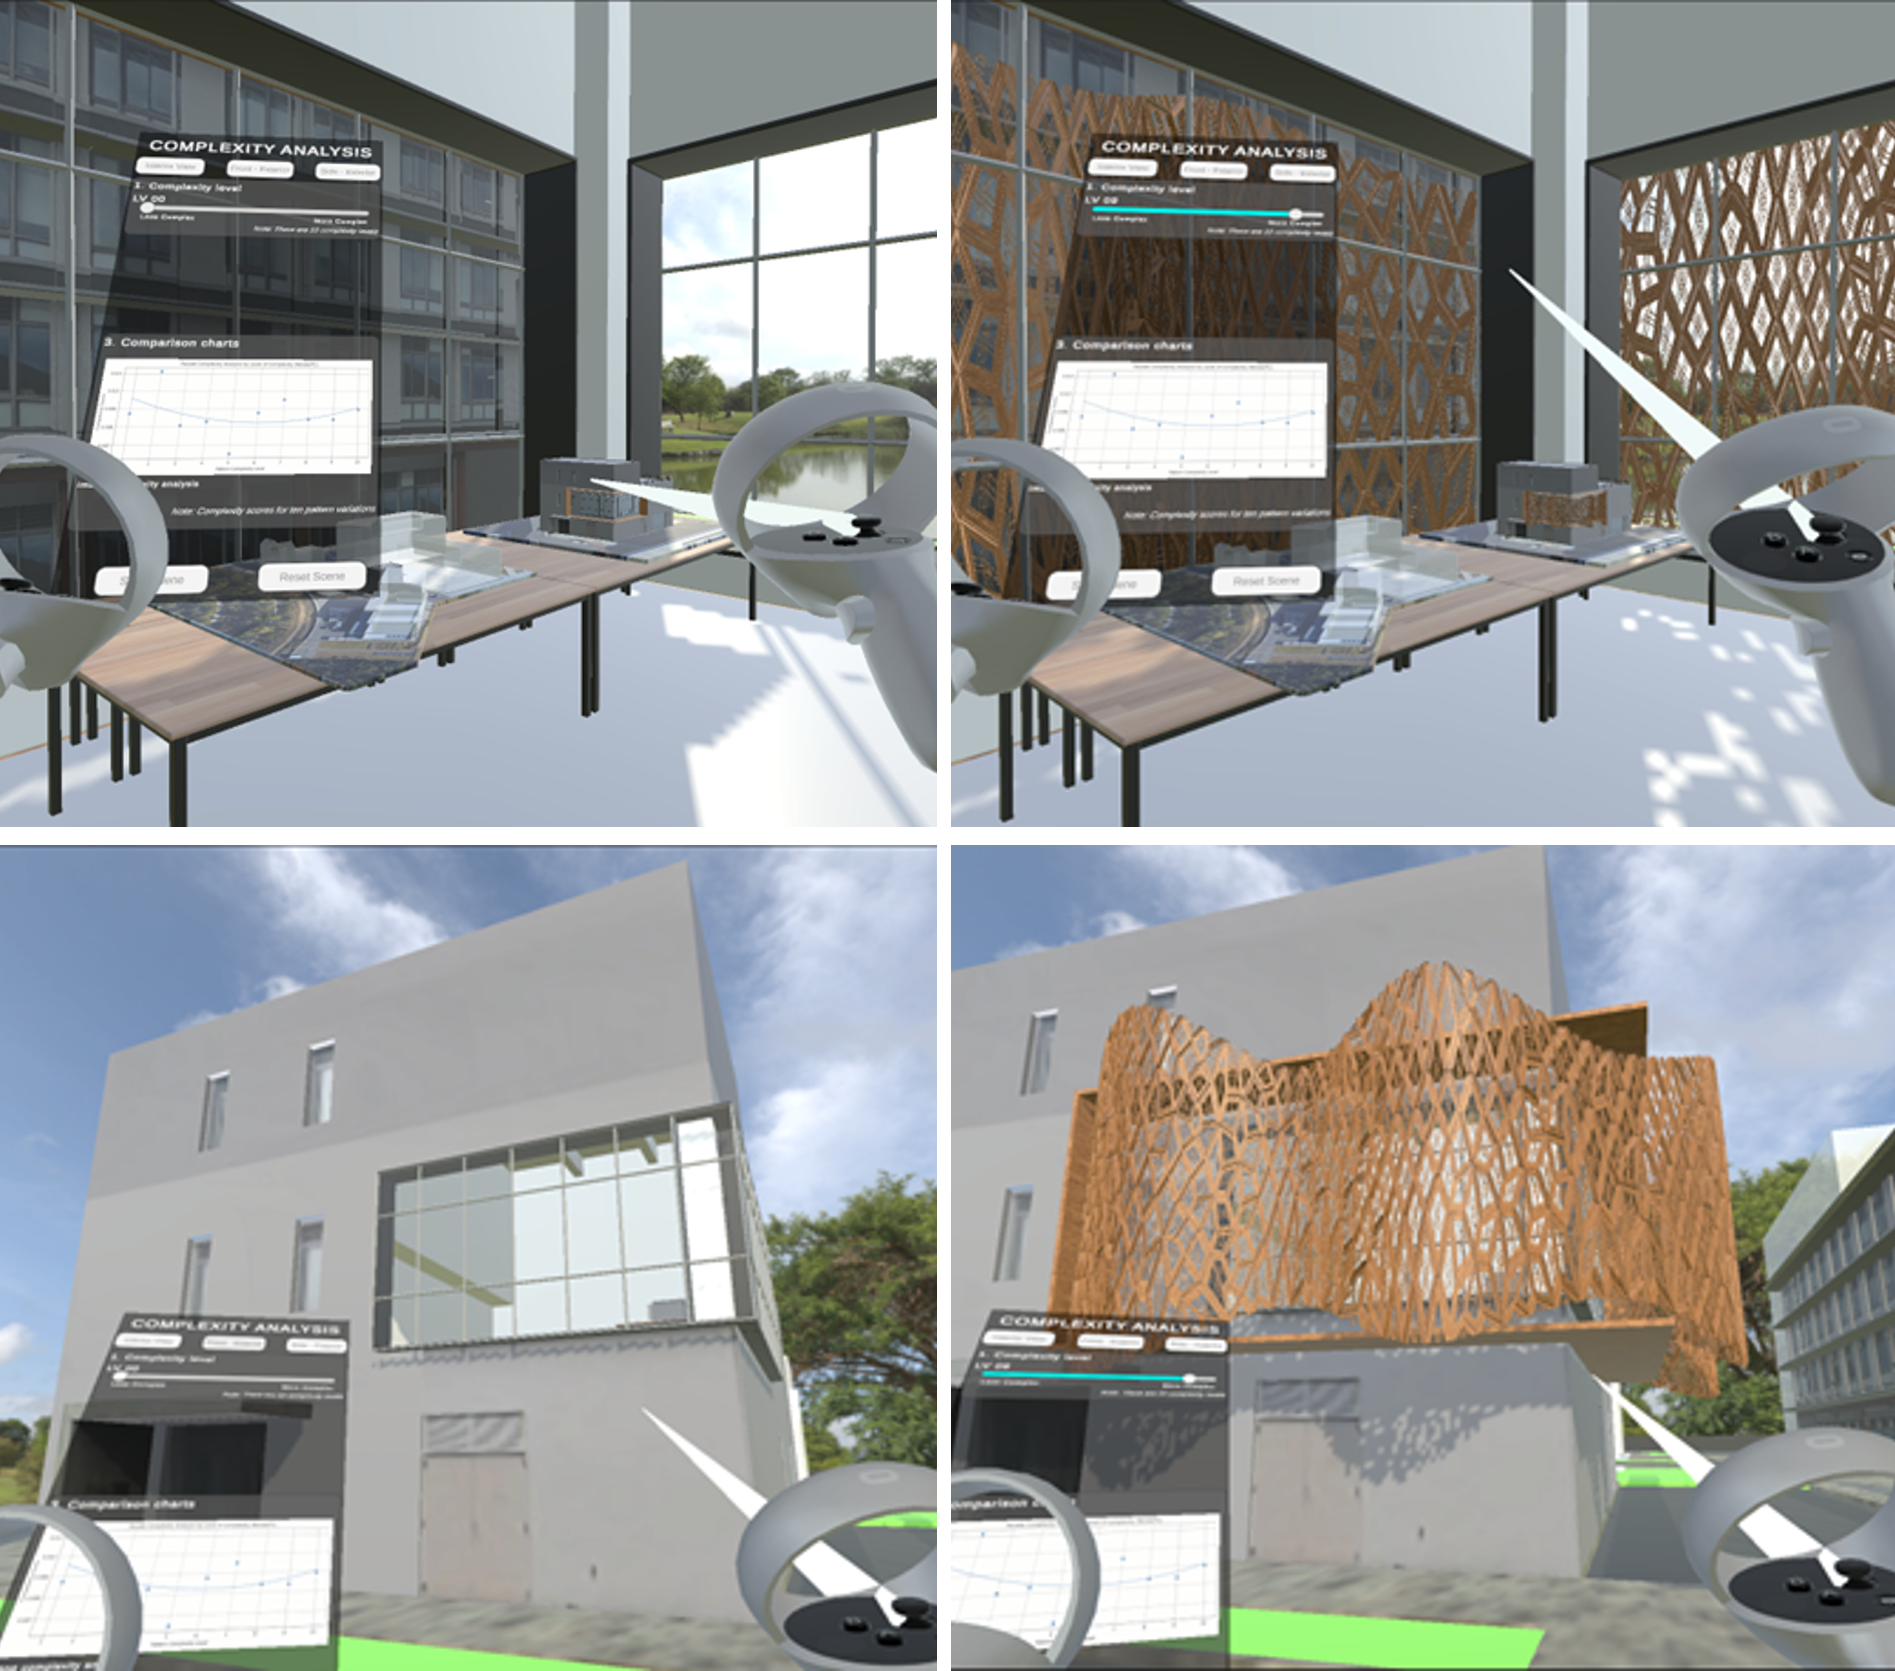
\includegraphics[width= \linewidth]{Images/VRInteriorExterior}
                \caption{Comparison side by side of the VR simulation of interior and exterior of existing laboratory building used for experiment (Left) and VR Simulation of facade variation (Right) used for complexity Analysis.}
                \label{fig:VRInteriorExterior}
            \end{figure}

            %% Figure of VR interface
            \begin{table*}[htb]
                \centering
                \small
                \begin{tabular}{c}
                    %Top cell
                    % Optimization Flowchart
                    \begin{minipage}{\textwidth}
                        \centering
                          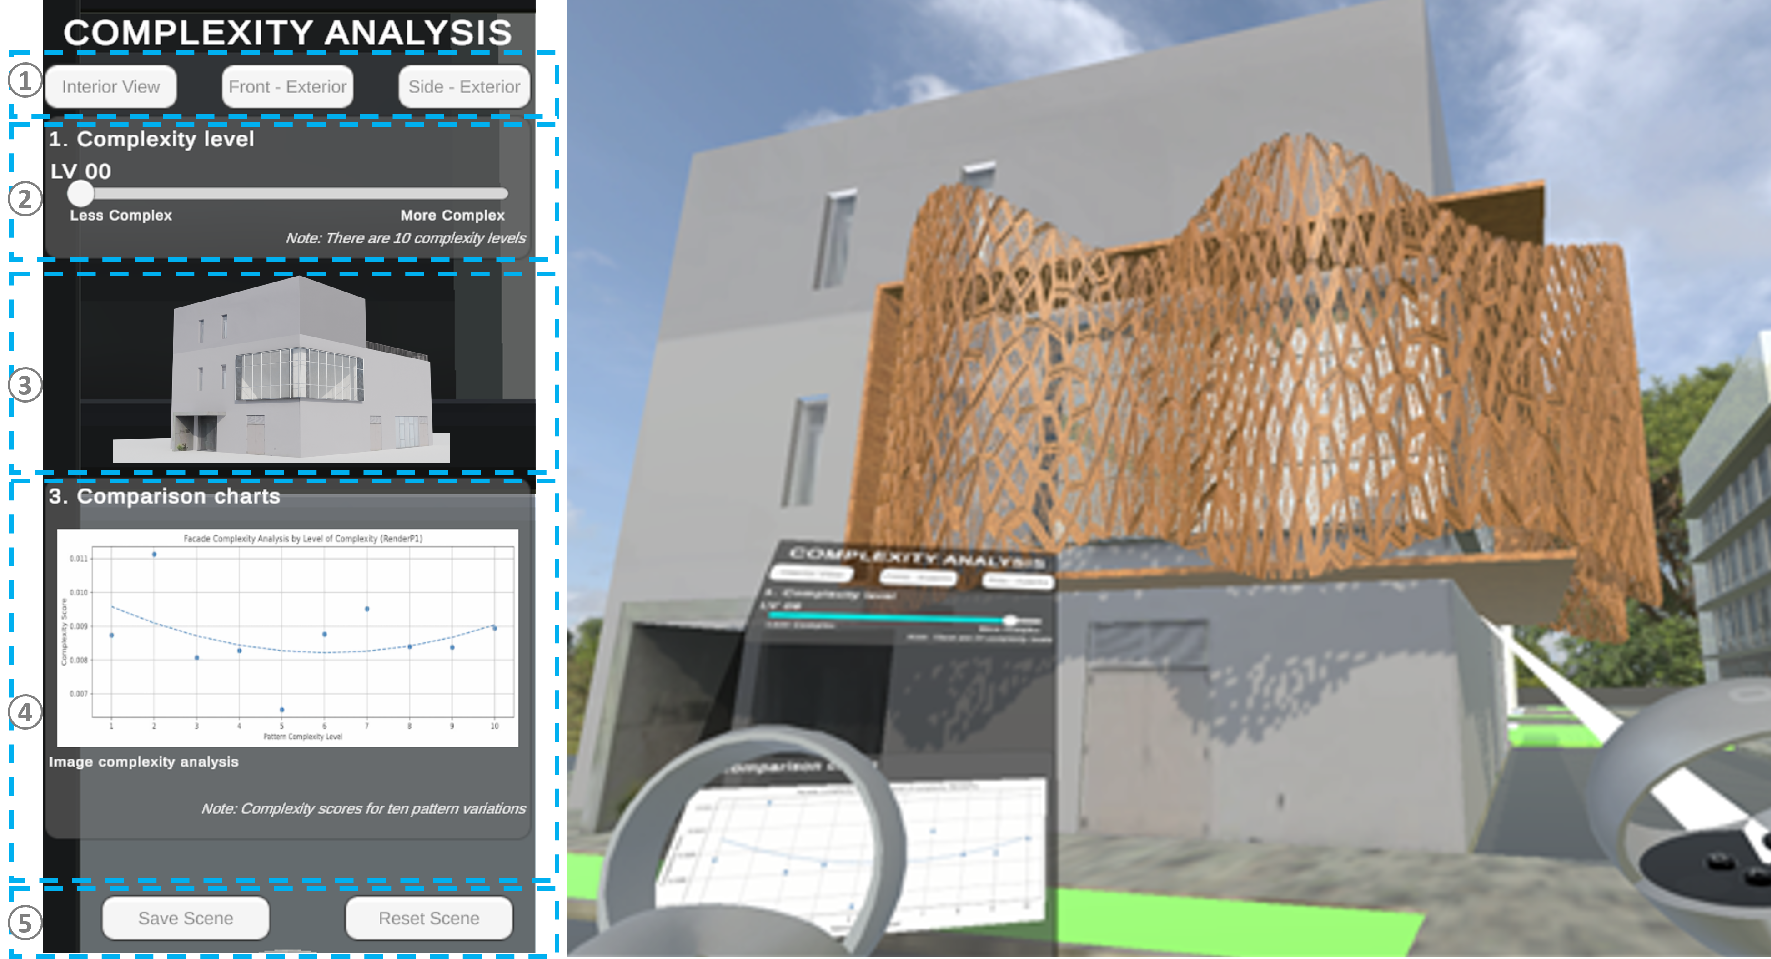
\includegraphics[width= \linewidth]{Images/VRInterface}
                        \captionof{figure}{VR interface for Complexity tolerance analysis in facade design. Predetermined cameras(1), Slider with variations of facades by level of complexity(2), Render preview of building with facade design (3), Comparison scatter graph with individual complexity scores of facade variations (4), Save and reset buttons (5) also used to transition among the three patterns.}
                        \label{fig:VRinterface}
                    \end{minipage}
                \end{tabular}
            \end{table*}

        \subsubsection{VR integration and data visualization interface}
        \label{subsubsec:VR_integration}
        %%Define the sections of the VR interface and how information is displayed
        %\subsubsection{VR integration and data visualization interface}
%\label{subsubsec:VR_integration}
%%Define the sections of the VR interface and how information is displayed
%\input{Text/VR_integration}


The goal of this component is to integrate the virtual environment from the `3D Modeling and Environment Setup' with data from the CICA complexity analysis (Figure~\ref{fig:MethodologyFlowchart}, element 3).
This module features an immersive `VR simulation' and a `data visualization interface' that allows users to explore and interact with the building's interior and exterior, visualize its context, and manipulate facade variations (Figure~\ref{fig:VRinterface}).

The `VR simulation,' developed using Unity (v.2022.2.21f1) and accessible through a Head-Mounted Display (HMD) like the Oculus Quest 2, this software was chosen for its robust VR support, pre-built templates, and seamless integration with Python and C\#, enhancing simulation interactivity and data handling.

%!Vr interface
The VR data visualization interface provides real-time feedback on facade variations, facilitating data collection on user response to varying levels of facade complexity.
Structured into five key sections—Viewpoint Navigation, Facade Variation Slider, Facade Render Preview, CICA Scores Comparative Analysis Charts, and Utility Functions (labeled 1 to 5 in Figure~\ref{fig:VRinterface})—it enhances usability and interpretability, thereby optimizing the facade selection process.







    \subsection{Experiment design}
    \label{subsec:Experiment_design}
    %%Task description, stage 1 to 3 with survey
    %\subsection{Experiment design}
%    \label{subsection:Experiment_design}
%    %%Task description, stage 1 to 3 with survey
%    %\subsection{Experiment design}
%    \label{subsection:Experiment_design}
%    %%Task description, stage 1 to 3 with survey
%    %\subsection{Experiment design}
%    \label{subsection:Experiment_design}
%    %%Task description, stage 1 to 3 with survey
%    \input{Text/ExperimentDesign}

With the VR system now comprehensively detailed, we transition into the experiment design phase, where we explore how this innovative virtual reality environment, equipped with the Computational Image Complexity Analysis (CICA) system-derived complexity data, will be utilized to investigate participants' responses to facade complexity variations.

This marks a pivotal stage in our study, where theory and technology converge to provide valuable insights into architectural complexity preferences.

The experiment is designed to comprehensively gauge participants' reactions to increasingly complex facade variations within immersive Virtual Reality simulations.
This process employs a Head-Mounted Display (HMD) and aims to quantitatively and qualitatively measure users' tolerance levels towards intricate facade designs (refer to Figure\ref{fig:ExperimentFlowchart}).

Conducted in our laboratory situated within the Architectural Environment Research Building, known as Building HE20, on the Itoshima campus of Kyushu University in Fukuoka, Japan, the experiment unfolds across three distinct stages: the `VR Interaction' stage, the `Screen-Based Ranking' stage, and the `Post-Experiment Survey' stage.

%% Figure Experiment Design flowchart
    \begin{figure}[htb]
      \centering
      % trim=left 190 down 250 right 150 top5
      \includegraphics[width= \linewidth, trim=0 0 0 0, clip]{Images/FlowchartExperiment}
      \caption{Flowchart illustrating the Experiment design stages, depicting the VR interaction stage, the Screen-based ranking stage and the Post-experiment survey.}
      \label{fig:ExperimentFlowchart}
    \end{figure}

%!VR interaction stage

In the initial stage of the experiment, participants were introduced to a Virtual Reality simulation that faithfully replicated the actual laboratory and building where they were invited to take part (Figure\ref{fig:VRInteriorExterior}).
Within this immersive environment, participants faced a distinctive challenge.
Their task was to select the most comfortable facade variation from a range of options presented in the virtual setting.

This scenario presented an intriguing question: if the laboratory were to become their permanent workplace or study location, how would participants choose a facade that would enhance their daily experience of entering the building and working within its confines, making it more comfortable and engaging?.

Participants were granted the freedom to incorporate their personal preferences into their final decisions, with a primary emphasis on enhancing workplace comfort.

To address this facade design selection challenge, participants were tasked with evaluating and selecting their preferred facade from three distinct patterns, each featuring ten variations labeled by complexity level (see \ref{sec:AnnexVariations}).
These patterns were presented in a randomized order to ensure unbiased results and were easily accessible as separate stages through the VR interface.

To provide participants with a heightened sense of realism and immersion, a section of the laboratory was cleared to allow them to physically move around within the virtual simulation of the lab.
This enabled them to gain a deeper understanding of how each facade variation would impact their environment.

This stage of the experiment yielded valuable insights into participants' complexity tolerance levels, extracted from their recorded selections of the facade variations they found most comfortable.


%! Screen-based ranking stage

After the conclusion of each of the three pattern stages in the VR system, participants proceeded to the `Screen-Based Ranking' stage of the experiment.

The primary objective of this stage was to assess the accuracy of the `Computational Image Complexity Analysis' (CICA) system in evaluating the complexity of facade variations in comparison to the perceptions of the participants.

In this stage, participants were presented with the same set of 10 facade variations that had been processed by the CICA system.
However, this time, the presentation format shifted to a screen-based interface, and participants used a mouse and keyboard to navigate through the images of the facade variations.

Their task was to independently analyze these variations and arrange them according to their personal judgments of complexity.
Participants were specifically instructed to disregard any aesthetic preferences when ranking the facades and concentrate solely on the degree of complexity, arranging them from the least complex (level 1) to the most complex (level 10).

This stage of the experiment was repeated three times, once for each of the three patterns.
The responses from participants were meticulously recorded and later used for evaluating the alignment between the participants' ranking assessments and those generated by the CICA system.

The primary goal of this analysis was to ascertain if there existed any notable disparities between the CICA system's rankings and the perceptions of the participants.
By scrutinizing the results of this ranking comparison, the study aimed to refine the Complexity Tolerance Metric derived from the first stage, adjusting it based on the margin of error resulting from the deviation observed in the second stage.
This refined metric provides a more precise basis for forecasting future trends in architectural construction, facilitating informed conclusions.

%! Post-experiment survey stage

The third and final stage of the experiment, known as the `Post-interaction Survey' stage, takes place after participants have completed both the Facade design selection task in the `VR interaction stage' and the facade variation ranking task in the `Screen-based ranking stage' for all three patterns.

This survey comprises 15 questions categorized into two sections: `Participant Background' and `Complexity Perception.'

The survey, provided in detail in \ref{sec:Annexsurvey}, serves a dual purpose.
Firstly, it aims to gather insights into the participants' professional backgrounds, including any prior experience they may have in addressing facade design-related challenges.
Secondly, it seeks to understand participants' perceptions of complexity in building design, shedding light on the decision-making processes that underlie their choices during the experiment.

The `Background section' encompasses 5 multiple-choice questions designed to identify participants' professional backgrounds and their previous involvement in solving facade design problems.

In contrast, the `Complexity perception section' features 10 questions measured on a 7-point Likert scale.
These questions delve into participants' qualitative perceptions of complexity when assessing a building.
Additionally, they help identify the key factors that influence their selection of a particular facade variation.

%! Metrics purpose

In summary, the comprehensive design of our experiment, consisting of three distinct stages - the `VR Interaction' stage, the `Screen-Based Ranking' stage, and the `Post-Experiment Survey' stage, is aimed at providing a multifaceted understanding of user tolerance for complex facades and its implications for future construction trends.

By integrating the quantitative data from the VR system, the ranking comparisons from the screen-based stage, and the qualitative responses from the survey, we can form a comprehensive understanding of user tolerance for complex facades.
We can also identify the drivers behind participants' preferences, shedding light on the evolving trends in future construction.

This combined analysis positions us to answer the core research question: What degree of complexity within facade design, would users tolerate and accept for a building, and what insights do their preferences provide for future architectural trends?' By combining quantitative and qualitative findings, we aim to provide a nuanced perspective that contributes to the discourse on architectural complexity and its implications for contemporary design and construction.





With the VR system now comprehensively detailed, we transition into the experiment design phase, where we explore how this innovative virtual reality environment, equipped with the Computational Image Complexity Analysis (CICA) system-derived complexity data, will be utilized to investigate participants' responses to facade complexity variations.

This marks a pivotal stage in our study, where theory and technology converge to provide valuable insights into architectural complexity preferences.

The experiment is designed to comprehensively gauge participants' reactions to increasingly complex facade variations within immersive Virtual Reality simulations.
This process employs a Head-Mounted Display (HMD) and aims to quantitatively and qualitatively measure users' tolerance levels towards intricate facade designs (refer to Figure\ref{fig:ExperimentFlowchart}).

Conducted in our laboratory situated within the Architectural Environment Research Building, known as Building HE20, on the Itoshima campus of Kyushu University in Fukuoka, Japan, the experiment unfolds across three distinct stages: the `VR Interaction' stage, the `Screen-Based Ranking' stage, and the `Post-Experiment Survey' stage.

%% Figure Experiment Design flowchart
    \begin{figure}[htb]
      \centering
      % trim=left 190 down 250 right 150 top5
      \includegraphics[width= \linewidth, trim=0 0 0 0, clip]{Images/FlowchartExperiment}
      \caption{Flowchart illustrating the Experiment design stages, depicting the VR interaction stage, the Screen-based ranking stage and the Post-experiment survey.}
      \label{fig:ExperimentFlowchart}
    \end{figure}

%!VR interaction stage

In the initial stage of the experiment, participants were introduced to a Virtual Reality simulation that faithfully replicated the actual laboratory and building where they were invited to take part (Figure\ref{fig:VRInteriorExterior}).
Within this immersive environment, participants faced a distinctive challenge.
Their task was to select the most comfortable facade variation from a range of options presented in the virtual setting.

This scenario presented an intriguing question: if the laboratory were to become their permanent workplace or study location, how would participants choose a facade that would enhance their daily experience of entering the building and working within its confines, making it more comfortable and engaging?.

Participants were granted the freedom to incorporate their personal preferences into their final decisions, with a primary emphasis on enhancing workplace comfort.

To address this facade design selection challenge, participants were tasked with evaluating and selecting their preferred facade from three distinct patterns, each featuring ten variations labeled by complexity level (see \ref{sec:AnnexVariations}).
These patterns were presented in a randomized order to ensure unbiased results and were easily accessible as separate stages through the VR interface.

To provide participants with a heightened sense of realism and immersion, a section of the laboratory was cleared to allow them to physically move around within the virtual simulation of the lab.
This enabled them to gain a deeper understanding of how each facade variation would impact their environment.

This stage of the experiment yielded valuable insights into participants' complexity tolerance levels, extracted from their recorded selections of the facade variations they found most comfortable.


%! Screen-based ranking stage

After the conclusion of each of the three pattern stages in the VR system, participants proceeded to the `Screen-Based Ranking' stage of the experiment.

The primary objective of this stage was to assess the accuracy of the `Computational Image Complexity Analysis' (CICA) system in evaluating the complexity of facade variations in comparison to the perceptions of the participants.

In this stage, participants were presented with the same set of 10 facade variations that had been processed by the CICA system.
However, this time, the presentation format shifted to a screen-based interface, and participants used a mouse and keyboard to navigate through the images of the facade variations.

Their task was to independently analyze these variations and arrange them according to their personal judgments of complexity.
Participants were specifically instructed to disregard any aesthetic preferences when ranking the facades and concentrate solely on the degree of complexity, arranging them from the least complex (level 1) to the most complex (level 10).

This stage of the experiment was repeated three times, once for each of the three patterns.
The responses from participants were meticulously recorded and later used for evaluating the alignment between the participants' ranking assessments and those generated by the CICA system.

The primary goal of this analysis was to ascertain if there existed any notable disparities between the CICA system's rankings and the perceptions of the participants.
By scrutinizing the results of this ranking comparison, the study aimed to refine the Complexity Tolerance Metric derived from the first stage, adjusting it based on the margin of error resulting from the deviation observed in the second stage.
This refined metric provides a more precise basis for forecasting future trends in architectural construction, facilitating informed conclusions.

%! Post-experiment survey stage

The third and final stage of the experiment, known as the `Post-interaction Survey' stage, takes place after participants have completed both the Facade design selection task in the `VR interaction stage' and the facade variation ranking task in the `Screen-based ranking stage' for all three patterns.

This survey comprises 15 questions categorized into two sections: `Participant Background' and `Complexity Perception.'

The survey, provided in detail in \ref{sec:Annexsurvey}, serves a dual purpose.
Firstly, it aims to gather insights into the participants' professional backgrounds, including any prior experience they may have in addressing facade design-related challenges.
Secondly, it seeks to understand participants' perceptions of complexity in building design, shedding light on the decision-making processes that underlie their choices during the experiment.

The `Background section' encompasses 5 multiple-choice questions designed to identify participants' professional backgrounds and their previous involvement in solving facade design problems.

In contrast, the `Complexity perception section' features 10 questions measured on a 7-point Likert scale.
These questions delve into participants' qualitative perceptions of complexity when assessing a building.
Additionally, they help identify the key factors that influence their selection of a particular facade variation.

%! Metrics purpose

In summary, the comprehensive design of our experiment, consisting of three distinct stages - the `VR Interaction' stage, the `Screen-Based Ranking' stage, and the `Post-Experiment Survey' stage, is aimed at providing a multifaceted understanding of user tolerance for complex facades and its implications for future construction trends.

By integrating the quantitative data from the VR system, the ranking comparisons from the screen-based stage, and the qualitative responses from the survey, we can form a comprehensive understanding of user tolerance for complex facades.
We can also identify the drivers behind participants' preferences, shedding light on the evolving trends in future construction.

This combined analysis positions us to answer the core research question: What degree of complexity within facade design, would users tolerate and accept for a building, and what insights do their preferences provide for future architectural trends?' By combining quantitative and qualitative findings, we aim to provide a nuanced perspective that contributes to the discourse on architectural complexity and its implications for contemporary design and construction.





With the VR system now comprehensively detailed, we transition into the experiment design phase, where we explore how this innovative virtual reality environment, equipped with the Computational Image Complexity Analysis (CICA) system-derived complexity data, will be utilized to investigate participants' responses to facade complexity variations.

This marks a pivotal stage in our study, where theory and technology converge to provide valuable insights into architectural complexity preferences.

The experiment is designed to comprehensively gauge participants' reactions to increasingly complex facade variations within immersive Virtual Reality simulations.
This process employs a Head-Mounted Display (HMD) and aims to quantitatively and qualitatively measure users' tolerance levels towards intricate facade designs (refer to Figure\ref{fig:ExperimentFlowchart}).

Conducted in our laboratory situated within the Architectural Environment Research Building, known as Building HE20, on the Itoshima campus of Kyushu University in Fukuoka, Japan, the experiment unfolds across three distinct stages: the `VR Interaction' stage, the `Screen-Based Ranking' stage, and the `Post-Experiment Survey' stage.

%% Figure Experiment Design flowchart
    \begin{figure}[htb]
      \centering
      % trim=left 190 down 250 right 150 top5
      \includegraphics[width= \linewidth, trim=0 0 0 0, clip]{Images/FlowchartExperiment}
      \caption{Flowchart illustrating the Experiment design stages, depicting the VR interaction stage, the Screen-based ranking stage and the Post-experiment survey.}
      \label{fig:ExperimentFlowchart}
    \end{figure}

%!VR interaction stage

In the initial stage of the experiment, participants were introduced to a Virtual Reality simulation that faithfully replicated the actual laboratory and building where they were invited to take part (Figure\ref{fig:VRInteriorExterior}).
Within this immersive environment, participants faced a distinctive challenge.
Their task was to select the most comfortable facade variation from a range of options presented in the virtual setting.

This scenario presented an intriguing question: if the laboratory were to become their permanent workplace or study location, how would participants choose a facade that would enhance their daily experience of entering the building and working within its confines, making it more comfortable and engaging?.

Participants were granted the freedom to incorporate their personal preferences into their final decisions, with a primary emphasis on enhancing workplace comfort.

To address this facade design selection challenge, participants were tasked with evaluating and selecting their preferred facade from three distinct patterns, each featuring ten variations labeled by complexity level (see \ref{sec:AnnexVariations}).
These patterns were presented in a randomized order to ensure unbiased results and were easily accessible as separate stages through the VR interface.

To provide participants with a heightened sense of realism and immersion, a section of the laboratory was cleared to allow them to physically move around within the virtual simulation of the lab.
This enabled them to gain a deeper understanding of how each facade variation would impact their environment.

This stage of the experiment yielded valuable insights into participants' complexity tolerance levels, extracted from their recorded selections of the facade variations they found most comfortable.


%! Screen-based ranking stage

After the conclusion of each of the three pattern stages in the VR system, participants proceeded to the `Screen-Based Ranking' stage of the experiment.

The primary objective of this stage was to assess the accuracy of the `Computational Image Complexity Analysis' (CICA) system in evaluating the complexity of facade variations in comparison to the perceptions of the participants.

In this stage, participants were presented with the same set of 10 facade variations that had been processed by the CICA system.
However, this time, the presentation format shifted to a screen-based interface, and participants used a mouse and keyboard to navigate through the images of the facade variations.

Their task was to independently analyze these variations and arrange them according to their personal judgments of complexity.
Participants were specifically instructed to disregard any aesthetic preferences when ranking the facades and concentrate solely on the degree of complexity, arranging them from the least complex (level 1) to the most complex (level 10).

This stage of the experiment was repeated three times, once for each of the three patterns.
The responses from participants were meticulously recorded and later used for evaluating the alignment between the participants' ranking assessments and those generated by the CICA system.

The primary goal of this analysis was to ascertain if there existed any notable disparities between the CICA system's rankings and the perceptions of the participants.
By scrutinizing the results of this ranking comparison, the study aimed to refine the Complexity Tolerance Metric derived from the first stage, adjusting it based on the margin of error resulting from the deviation observed in the second stage.
This refined metric provides a more precise basis for forecasting future trends in architectural construction, facilitating informed conclusions.

%! Post-experiment survey stage

The third and final stage of the experiment, known as the `Post-interaction Survey' stage, takes place after participants have completed both the Facade design selection task in the `VR interaction stage' and the facade variation ranking task in the `Screen-based ranking stage' for all three patterns.

This survey comprises 15 questions categorized into two sections: `Participant Background' and `Complexity Perception.'

The survey, provided in detail in \ref{sec:Annexsurvey}, serves a dual purpose.
Firstly, it aims to gather insights into the participants' professional backgrounds, including any prior experience they may have in addressing facade design-related challenges.
Secondly, it seeks to understand participants' perceptions of complexity in building design, shedding light on the decision-making processes that underlie their choices during the experiment.

The `Background section' encompasses 5 multiple-choice questions designed to identify participants' professional backgrounds and their previous involvement in solving facade design problems.

In contrast, the `Complexity perception section' features 10 questions measured on a 7-point Likert scale.
These questions delve into participants' qualitative perceptions of complexity when assessing a building.
Additionally, they help identify the key factors that influence their selection of a particular facade variation.

%! Metrics purpose

In summary, the comprehensive design of our experiment, consisting of three distinct stages - the `VR Interaction' stage, the `Screen-Based Ranking' stage, and the `Post-Experiment Survey' stage, is aimed at providing a multifaceted understanding of user tolerance for complex facades and its implications for future construction trends.

By integrating the quantitative data from the VR system, the ranking comparisons from the screen-based stage, and the qualitative responses from the survey, we can form a comprehensive understanding of user tolerance for complex facades.
We can also identify the drivers behind participants' preferences, shedding light on the evolving trends in future construction.

This combined analysis positions us to answer the core research question: What degree of complexity within facade design, would users tolerate and accept for a building, and what insights do their preferences provide for future architectural trends?' By combining quantitative and qualitative findings, we aim to provide a nuanced perspective that contributes to the discourse on architectural complexity and its implications for contemporary design and construction.





            %!Figure of Results for CICA in History Arch Style
            %facade Complexity analysis graph by year and architectural style
            \begin{figure*}[htb]
          \centering
          \includegraphics[width= \linewidth]{Graphs/complexitygraph}
          \caption{Scatter graph showcasing quantitative image complexity analysis scores for building images categorized by historical timeline and architectural style, with an overlaid trendline highlighting the evolving trend towards increased complexity.}
          \label{fig:HistoricalComplexityGraph}
     \end{figure*}

\section{Results}
\label{sec:Results}
%% Results should be clear and concise.
%!\section{Results}
%\label{sec:Results}
%%!\section{Results}
%\label{sec:Results}
%%!\section{Results}
%\label{sec:Results}
%\input{text/ResultsIntro.tex}

%=============================
%%% Results should be clear and concise.
%Report the results of the study
%Report main findings concisely in a logical order

%===============

In this section, we embark on a journey through the outcomes of our extensive study.
Our research was designed to delve into the intricate world of architectural complexity, investigating how users perceive and respond to increasing levels of complexity in facade design.
Our primary aim was to measure their tolerance for intricate facade designs, with the ultimate goal of contributing valuable insights to the ongoing discourse on future construction trends.

Building upon the methodologies outlined in the previous section, we present our findings in a structured manner.
The results are divided into two distinct sections: firstly, the outcomes of our `Computational Image Complexity Analysis' (CICA) application across different epochs and architectural styles (see Figure \ref{fig:HistoricalComplexityGraph}), and secondly, the results derived from our experiment gauging user responses to complex facades.

However, it's essential to recognize that every research endeavor carries its unique set of limitations, and our study is no exception.
In the spirit of transparency, we candidly acknowledge these limitations, which we will address.
Nevertheless, the following subsections, which meticulously analyze our results, were arranged in accordance with the core themes and research questions that guided our inquiry.





%=============================
%%% Results should be clear and concise.
%Report the results of the study
%Report main findings concisely in a logical order

%===============

In this section, we embark on a journey through the outcomes of our extensive study.
Our research was designed to delve into the intricate world of architectural complexity, investigating how users perceive and respond to increasing levels of complexity in facade design.
Our primary aim was to measure their tolerance for intricate facade designs, with the ultimate goal of contributing valuable insights to the ongoing discourse on future construction trends.

Building upon the methodologies outlined in the previous section, we present our findings in a structured manner.
The results are divided into two distinct sections: firstly, the outcomes of our `Computational Image Complexity Analysis' (CICA) application across different epochs and architectural styles (see Figure \ref{fig:HistoricalComplexityGraph}), and secondly, the results derived from our experiment gauging user responses to complex facades.

However, it's essential to recognize that every research endeavor carries its unique set of limitations, and our study is no exception.
In the spirit of transparency, we candidly acknowledge these limitations, which we will address.
Nevertheless, the following subsections, which meticulously analyze our results, were arranged in accordance with the core themes and research questions that guided our inquiry.





%=============================
%%% Results should be clear and concise.
%Report the results of the study
%Report main findings concisely in a logical order

%===============

In this section, we embark on a journey through the outcomes of our extensive study.
Our research was designed to delve into the intricate world of architectural complexity, investigating how users perceive and respond to increasing levels of complexity in facade design.
Our primary aim was to measure their tolerance for intricate facade designs, with the ultimate goal of contributing valuable insights to the ongoing discourse on future construction trends.

Building upon the methodologies outlined in the previous section, we present our findings in a structured manner.
The results are divided into two distinct sections: firstly, the outcomes of our `Computational Image Complexity Analysis' (CICA) application across different epochs and architectural styles (see Figure \ref{fig:HistoricalComplexityGraph}), and secondly, the results derived from our experiment gauging user responses to complex facades.

However, it's essential to recognize that every research endeavor carries its unique set of limitations, and our study is no exception.
In the spirit of transparency, we candidly acknowledge these limitations, which we will address.
Nevertheless, the following subsections, which meticulously analyze our results, were arranged in accordance with the core themes and research questions that guided our inquiry.






    \subsection{Computational Image complexity Analysis (CICA) system results across architectural styles}
    \label{subsec:ResultsComplexityImageAnalysishistory}
    %!\subsection{Quantitative complexity Analysis}
%    \label{subsec:ComplexityImageAnalysis}
%    %!\subsection{Quantitative complexity Analysis}
%    \label{subsec:ComplexityImageAnalysis}
%    %!\subsection{Quantitative complexity Analysis}
%    \label{subsec:ComplexityImageAnalysis}
%    \input{Text/ResultsImageComplexityAnalysisHistory.tex}
%% Figure of Complexity graph


We have previously discussed the argument that the architectural evolution, throughout history, has been characterized by a continual interplay between simplicity and complexity.
This notion has been substantiated by our exploration of the theoretical definitions and varied approaches to facades and ornamentation within the context of prominent architectural styles and the perspectives of their eminent architects.

Our literature review has consistently pointed towards a prevailing trend in contemporary architecture, suggesting a resurgence of complexity in architectural design.
However, to ensure our findings are not purely subjective or biased towards this conclusion, we have conducted a quantitative analysis using the Computational Image Complexity Analysis (CICA) system.
This rigorous analysis method utilizes input images of the most iconic and representative buildings from various epochs and styles.

The results are visually depicted in Figure\ref{fig:HistoricalComplexityGraph}, where a discernible upward trendline towards complexity emerges, particularly noticeable since the late 20th century.

%!facade Complexity analysis graph by year and architectural style
     \begin{figure*}[htb]
          \centering
          \includegraphics[width= \linewidth]{Graphs/complexitygraph}
          \caption{Scatter graph showcasing quantitative image complexity analysis scores for building images categorized by historical timeline and architectural style, with an overlaid trendline highlighting the evolving trend towards increased complexity.}
          \label{fig:HistoricalComplexityGraph}
     \end{figure*}










%% Figure of Complexity graph


We have previously discussed the argument that the architectural evolution, throughout history, has been characterized by a continual interplay between simplicity and complexity.
This notion has been substantiated by our exploration of the theoretical definitions and varied approaches to facades and ornamentation within the context of prominent architectural styles and the perspectives of their eminent architects.

Our literature review has consistently pointed towards a prevailing trend in contemporary architecture, suggesting a resurgence of complexity in architectural design.
However, to ensure our findings are not purely subjective or biased towards this conclusion, we have conducted a quantitative analysis using the Computational Image Complexity Analysis (CICA) system.
This rigorous analysis method utilizes input images of the most iconic and representative buildings from various epochs and styles.

The results are visually depicted in Figure\ref{fig:HistoricalComplexityGraph}, where a discernible upward trendline towards complexity emerges, particularly noticeable since the late 20th century.

%!facade Complexity analysis graph by year and architectural style
     \begin{figure*}[htb]
          \centering
          \includegraphics[width= \linewidth]{Graphs/complexitygraph}
          \caption{Scatter graph showcasing quantitative image complexity analysis scores for building images categorized by historical timeline and architectural style, with an overlaid trendline highlighting the evolving trend towards increased complexity.}
          \label{fig:HistoricalComplexityGraph}
     \end{figure*}










%% Figure of Complexity graph


We have previously discussed the argument that the architectural evolution, throughout history, has been characterized by a continual interplay between simplicity and complexity.
This notion has been substantiated by our exploration of the theoretical definitions and varied approaches to facades and ornamentation within the context of prominent architectural styles and the perspectives of their eminent architects.

Our literature review has consistently pointed towards a prevailing trend in contemporary architecture, suggesting a resurgence of complexity in architectural design.
However, to ensure our findings are not purely subjective or biased towards this conclusion, we have conducted a quantitative analysis using the Computational Image Complexity Analysis (CICA) system.
This rigorous analysis method utilizes input images of the most iconic and representative buildings from various epochs and styles.

The results are visually depicted in Figure\ref{fig:HistoricalComplexityGraph}, where a discernible upward trendline towards complexity emerges, particularly noticeable since the late 20th century.

%!facade Complexity analysis graph by year and architectural style
     \begin{figure*}[htb]
          \centering
          \includegraphics[width= \linewidth]{Graphs/complexitygraph}
          \caption{Scatter graph showcasing quantitative image complexity analysis scores for building images categorized by historical timeline and architectural style, with an overlaid trendline highlighting the evolving trend towards increased complexity.}
          \label{fig:HistoricalComplexityGraph}
     \end{figure*}











    \subsection{Results of experiment on users response to complex facades}
    \label{subsec:ResultsExperiment}
    %\section{Results}
%\label{sec:Results}
%% Results should be clear and concise.

The experiment to test the hypothesis that participants in a virtual reality (VR) experiment would show a trend towards choosing complex environments over simple ones when given the task of identifying the more comfortable facade design, wa conducted at the Kyushu University campus in Fukuoka, Japan, over a period of 15 days, from October 12 to 30, 2023, during the work hours between 10:00 and 18:00.

A total of 10 participants took part in the experiment, primarily consisting of university students and faculty members.
The participants had diverse professional backgrounds, as shown in Figure \ref{fig:ParticipantBackgroundChart}, with over \(67\%\) being students from various faculties, approximately \(33\%\) having a construction background, and \(14\%\) reporting previous experience in facade design, as indicated in Figure \ref{fig:YearsExperienceChart}

%% Participant background chart and years of experience
    \begin{table*}[htb]
        \centering
        \small
        \begin{tabularx}{\textwidth}{X X}
            \centering
            % trim=left 0 down 50 right 0 top 50
            \includegraphics[width=\linewidth, trim=0 60 0 0]{Images/SurveyBackground}
            \captionof{figure}{This chart shows the professional backgrounds of participants involved in the facade design complexity analysis experiment.}
            \label{fig:SurveyBackgroundChart} &
            \centering
            \includegraphics[width=\linewidth, trim=0 60 0 0]{Images/SurveyExperience}
            \captionof{figure}{This chart displays the experience levels in facade design of participants for the study complexity analysis in building design.}
            \label{fig:SurveyYearsExperienceChart}
        \end{tabularx}
    \end{table*}

Regarding the first theme of analysis addressed during the `VR Interaction' stage, related to user tolerance to complex facade design, all participants completed the facade selection task for all three patterns, resulting in a total of 30 experiment sessions.
For each pattern, one answer was recorded based on the facade variation, labeled by the level of complexity, that the participant choose as the most comfortable.

%!Complexity level chosen bar chart
These outcomes were summarized in a bar chart referred to as `Complexity level Chosen graph' as depicted in Figure \ref{fig:ComplexityLevelChosenChart}.

    % Complexity level chosen Chart
    \begin{figure}[htb]
        \centering
        %trim=100 180 100 120, clip
        \includegraphics[width=\linewidth]{Images/ComplexityLevelChosenChart}
        \caption{Chart displaying participants' preferred complexity levels among the ten options during the VR simulation stage of the experiment for all three patterns.}
        \label{fig:ComplexityLevelChosenChart}
    \end{figure}

The Complexity chosen level results, depicted in the `Complexity level Chosen graph' in Figure \ref{fig:ComplexityLevelChosenChart}, showcased a diverse range of preferences among the 30 experiment sessions, with most of them allocated bellow the `level 5' of complexity and only five instances going above this line, returning overall an average of  complexity level \(3.9\) as the preferred one among the 10 levels defined for the facade variations for all three patterns.

The preferred complexity level depicted on this graph exhibited a wide distribution, as indicated by the current standard deviation of \(2.3\).

%!Complexity level chosen probability graph

The probability bell graph displayed in Figure \ref{fig:ProbabilityComplexitylevelChart} further illustrates the distribution of choices in the results, emphasizing that there is a \(40\%\) probability of a focus group selecting and answer close to the level 4 of complexity as defined by the facade variations with a standard deviation of \(11\%\)in predicting individual data points or outcomes.

     % Probability Chart and Complexity level per Pattern
    \begin{table*}[htb]
        \centering
        \small
        \begin{tabularx}{\textwidth}{X X}
            \centering
            \includegraphics[width=\linewidth, trim=0 0 0 20]{Images/ProbabilityPreferredComplexitylevel}
            \captionof{figure}{Scatter graph illustrating the probability distribution of preferred complexity levels for facade design across all three patterns, derived from data collected during the VR stage of the experiment.}
            \label{fig:ProbabilityComplexitylevelChart} &
            \centering
            \includegraphics[width=\linewidth, trim=0 0 0 20]{Images/PreferredComplexityLevelPerPattern}
            \captionof{figure}{Average preferred complexity level per pattern by participants during the VR simulation (Overall Mean complexity level = \(4.9\)).}
            \label{fig:ComplexityLevelPerPattern}
        \end{tabularx}
    \end{table*}

%% probability preferred complexity level Chart
%    \begin{figure}[htb]
%        \centering
%        \includegraphics[width=\linewidth]{Images/ProbabilityPreferredComplexitylevel}
%        \caption{Scatter graph illustrating the probability distribution of preferred complexity levels for facade design across all three patterns, derived from data collected during the VR stage of the experiment.}
%        \label{fig:ProbabilityComplexitylevelChart}
%    \end{figure}

%!Complexity level per pattern graph

Analyzing the average complexity level chosen per pattern (Figure \ref{fig:ComplexityLevelPerPattern}) revealed that the average choice across all patterns remains close to the overall average complexity level \(3.9\).

%===============Continue from here for the accuracy section

as radial graphs, referred to as "accuracy analysis graphs," as depicted in Figure \ref{fig:Accuracyscattergraph}.

 %% Figure Accuracy graph
    \begin{figure*}[htb]
      \centering
      \includegraphics[width= \linewidth, trim=0 0 0 0]{Images/ComplexityPerceptionPerLevel}
      \caption{This graph highlights participants' perception of complexity for the 10 variations within three patterns in contrast to the original ranking. It visually represents the differences between participants' perceived complexity and the initial rankings during the screen-based complexity assessment stage of the experiment.}
      \label{fig:ComplexityPerceptionPerLevel}
    \end{figure*}

In these graphs, the center serves as a reference point, representing the top recommendation provided by the optimization system for each specific site.
The coordinates of this center point vary for each site, reflecting the distinct optimal locations suggested by the system.
On the other hand, the participants' chosen locations are plotted on the graph, precisely indicating the positions they deemed most suitable for the new educational building within the boundaries of the site.

The placement of each participant's chosen location on the graph is based on its actual geographical coordinates, ensuring an accurate representation of their decision-making process.
The distance between each participant's chosen location and the center reflects the deviation error from the system's top recommendation, allowing for a clear assessment of how closely participants' choices align with the data-driven optimization results.

Furthermore, the orientation of each chosen location on the graph provides valuable insights into the direction in which participants opted to position the building, allowing for a comprehensive understanding of their decision-making rationale.
Overall, these accuracy analysis graphs present an actual representation of the chosen locations on the physical site, capturing both spatial proximity and directional preferences relative to the system's top recommendation.

The purpose of the analysis was to evaluate the reduction in the deviation error between the preferred SLP location recommended by our Multi-objective optimization (MOO) model and the location ultimately chosen by the experiment participants in both the ``screen-based'' and "VR interaction" stages of the experiment.

By analyzing the accuracy analysis graphs, the contribution of the VR system was determined by examining the vector resultant from the center point (top recommendation) to the participant's chosen location.
A reduction in the vector magnitude in the "VR answer" compared to the "screen-based answer" indicated an improvement percentage, while an increase represented a decline.
This analysis allowed us to quantify the impact of VR immersion on participants' decision-making accuracy in SLP design.

The accuracy analysis results, depicted in the "Accuracy improvement" bar chart in Figure \ref{fig:ImprovementChart}, showcased varying degrees of improvement among the 39 experiment sessions, with only three cases showing a decline.
On average, there was a \(48.3\%\) improvement among the participants.

The accuracy analysis results, illustrated in the "Accuracy improvement" bar chart (Figure \ref{fig:ImprovementChart}), revealed varying degrees of improvement among the 39 experiment sessions, with only three cases showing a decline.
On average, there was a significant \(48.3\%\) improvement among the participants.

    % Complexity perception Chart
    \begin{figure}[htb]
        \centering
        %trim=100 180 100 120, clip
        \includegraphics[width=\linewidth]{Images/ComplexityPerceptionChart}
        \caption{Chart depicting participants' complexity perception related to the three patterns. Insights into participants' perception of complexity concerning specific patterns during the screen-based complexity assessment phase of the experiment.}
        \label{fig:ComplexityPerceptionChart}
    \end{figure}

%! Post experiment survey results

The survey results provided additional insights into the influence of VR interaction and data-driven optimization for SLP. The ``influence perception'' section of the survey, depicted in Figure\ref{fig:PerceptionSatisfactionSurveyResults}, indicated that the system scored above 5 on a 7-point Likert scale for all questions, suggesting a positive influence of the VR strategy in introducing data-driven recommendations.
This finding aligned with the accuracy improvement percentage results observed in the accuracy analysis (Figure\ref{fig:ImprovementChart}).


  %% Complexity Perception Survey results
    \begin{table*}[htb]
        \centering
        \small
        \begin{tabularx}{\textwidth}{X X}
            \centering
            \includegraphics[width=\linewidth]{Images/SurveyPart1Complexity}
            \captionof{figure}{User Satisfaction section questions from User Survey of SLP System. \- (n = 17), 1 - strongly disagree, 7 - strongly agree}
            \label{fig:SurveyQuestions6-10} &
            \centering
            \includegraphics[width=\linewidth]{Images/SurveyPart2Complexity}
            \captionof{figure}{User-System Influence Perception section" questions. \- (n = 17), 1 - strongly disagree, 7 - strongly agree}
            \label{fig:SurveyQuestions11-15}
        \end{tabularx}
    \end{table*}


During post-experiment interviews, participants were asked for their opinions on the weight distribution used by the optimization model to balance the trade-offs between the three performance indicators.
The initial distribution decided for the system was set at 50, 30, and 20 for the respective indicators (see Table \ref{tab:PerformanceIndicators}).
While most participants maintained a consistent criteria for ranking the indicators, slight deviations from the predetermined weight distribution were observed.
Figure \ref{fig:PerformanceIndicatorweightChart} visually represents the average weight configuration suggested by the participants, demonstrating their individual preferences in adjusting the trade-off weights for each site.

Overall, the results support the initial hypothesis, indicating that VR has the potential to enhance the acceptance of data-driven design recommendations in SLP. However, the "user satisfaction" section of the survey, summarized in Figure \ref{fig:UsabilityChartSurvey}, revealed room for improvement in the user interface and experience, with scores above 4.5 on a 7-point Likert scale.
Notably, the areas of helpfulness and visualization enhancement ranked the lowest, despite initially being considered key advantages of the "VR interaction" system compared to the "screen-based" alternative.


\section{Discussion}
\label{sec:Discussion}
%% This should explore the significance of the results of the work, not repeat them. A combined Results and Discussion section is often appropriate. Avoid extensive citations and discussion of published literature.
%!\section{Discussion}
%\label{sec:Discussion}
%%% This should explore the significance of the results of the work, not repeat them. A combined Results and Discussion section is often appropriate. Avoid extensive citations and discussion of published literature.
%%%!\section{Discussion}
%\label{sec:Discussion}
%%% This should explore the significance of the results of the work, not repeat them. A combined Results and Discussion section is often appropriate. Avoid extensive citations and discussion of published literature.
%%%!\section{Discussion}
%\label{sec:Discussion}
%%% This should explore the significance of the results of the work, not repeat them. A combined Results and Discussion section is often appropriate. Avoid extensive citations and discussion of published literature.
%%\input{Text/Discussion}

Discussion on results of history analysis and how theory aligns with the computational image analysis.
Followed by a tuning of the level of complexity how we interpret the survey results to propose a graphical conclusion of an apparent complex facade inside the boundaries of tolerance given by the experiment participants.

%! Historical Analysis graph

Through Image Complexity Analysis, we assign a quantitative complexity value to these architectural images.
This complexity value is derived from a comprehensive examination of spatial intricacies, frequency patterns, and color information present within, based on the research strategy by Ishra et al\cite{Ishrat2020}.

By employing this quantitative approach, we aim to provide an objective measure of the shift from simplicity towards complexity in architecture, further strengthening the thesis of an impending era characterized by architectural intricacy and richness in facades and ornamentation.

This graphical representation unmistakably illustrates a growing inclination towards architecturally complex designs, further corroborating the conclusion drawn from our extensive literature review.
%=========
%
% Complexity of an image is governed by spatial, frequency and color information present in the image.\cite{Ishrat2020}
%
%Scanpath based image complexity analysis determines human visual behavior that could lead to development of interactive and intelligent systems.\cite{Ishrat2020}
%
%The objective of current research work is to establish the complexity of the given set of images while target objects are searched and to present analysis ofgaze search pattern.
%To achieve these objectives a remote gaze estimation and analysis model has been proposed for scanpath identification and analysis.\cite{Ishrat2020}


%! Experiment results discussions


Discussion on results of history analysis and how theory aligns with the computational image analysis.
Followed by a tuning of the level of complexity how we interpret the survey results to propose a graphical conclusion of an apparent complex facade inside the boundaries of tolerance given by the experiment participants.

%! Historical Analysis graph

Through Image Complexity Analysis, we assign a quantitative complexity value to these architectural images.
This complexity value is derived from a comprehensive examination of spatial intricacies, frequency patterns, and color information present within, based on the research strategy by Ishra et al\cite{Ishrat2020}.

By employing this quantitative approach, we aim to provide an objective measure of the shift from simplicity towards complexity in architecture, further strengthening the thesis of an impending era characterized by architectural intricacy and richness in facades and ornamentation.

This graphical representation unmistakably illustrates a growing inclination towards architecturally complex designs, further corroborating the conclusion drawn from our extensive literature review.
%=========
%
% Complexity of an image is governed by spatial, frequency and color information present in the image.\cite{Ishrat2020}
%
%Scanpath based image complexity analysis determines human visual behavior that could lead to development of interactive and intelligent systems.\cite{Ishrat2020}
%
%The objective of current research work is to establish the complexity of the given set of images while target objects are searched and to present analysis ofgaze search pattern.
%To achieve these objectives a remote gaze estimation and analysis model has been proposed for scanpath identification and analysis.\cite{Ishrat2020}


%! Experiment results discussions


Discussion on results of history analysis and how theory aligns with the computational image analysis.
Followed by a tuning of the level of complexity how we interpret the survey results to propose a graphical conclusion of an apparent complex facade inside the boundaries of tolerance given by the experiment participants.

%! Historical Analysis graph

Through Image Complexity Analysis, we assign a quantitative complexity value to these architectural images.
This complexity value is derived from a comprehensive examination of spatial intricacies, frequency patterns, and color information present within, based on the research strategy by Ishra et al\cite{Ishrat2020}.

By employing this quantitative approach, we aim to provide an objective measure of the shift from simplicity towards complexity in architecture, further strengthening the thesis of an impending era characterized by architectural intricacy and richness in facades and ornamentation.

This graphical representation unmistakably illustrates a growing inclination towards architecturally complex designs, further corroborating the conclusion drawn from our extensive literature review.
%=========
%
% Complexity of an image is governed by spatial, frequency and color information present in the image.\cite{Ishrat2020}
%
%Scanpath based image complexity analysis determines human visual behavior that could lead to development of interactive and intelligent systems.\cite{Ishrat2020}
%
%The objective of current research work is to establish the complexity of the given set of images while target objects are searched and to present analysis ofgaze search pattern.
%To achieve these objectives a remote gaze estimation and analysis model has been proposed for scanpath identification and analysis.\cite{Ishrat2020}


%! Experiment results discussions


    %\subsection{Future Trends and speculations}
    %\label{subsec:Futuretrends}
    %%!\subsection{Future Trends and speculations}
%!\label{subsec:Futuretrends}

%!==========================
%Speculate on the potential future trajectories of architectural design, digital fabrication, and mixed reality. Discuss how these trends might shape the built environment, and propose ideas for further research and exploration.
%!==========================

%!\subsection{Object-Oriented Ontology}
%!\label{subsec:ObjectOrientedOntology}
% add the concept of Object-Oriented. Using these concepts as basis. I want to express that the mr experiment is based on the idea that architecture as a tool should be invisible and confortable while in use. But it should  create emotion when seen as part of the landscape as a form of art to recapture the humand oriented city .

It may be cheaper and quicker to build a load-bearing brick wall, but
the High Tech architect will always prefer the steel frame and the lightweight metal panel because this is a technique more in tune with the spirit of the age.
He is committed to the idea that building must eventually catch up with the rest of technology, and he is determined to "drag building into the twentieth century".\cite{Davies1988}

Heideggers tool analysis states that as the tool is a tool it disappears in favor of some purpose he continues to explain that generally we don't notice equipment until it fails, like when An earthquake calls attention to the ground we walk or when a medical problem alerts us of the presence of organs that we have silently depended\cite{Harman2011}.
Harmans, Object-oriented ontology, borrows this concept to formulate its central claim that objects have hidden qualities and realities, and they withdraw from our understanding.\cite{Gage2015}
he idea that we live our lives on a layer of invisible equipment has significant ramifications for architecture, a discipline that produces the equipment on and in which we exist.\cite{Gage2015}

(Figure \ref{fig:complexornament})

%% Figure of Contemporary timeline
     \begin{figure*}[htb]
          \centering
          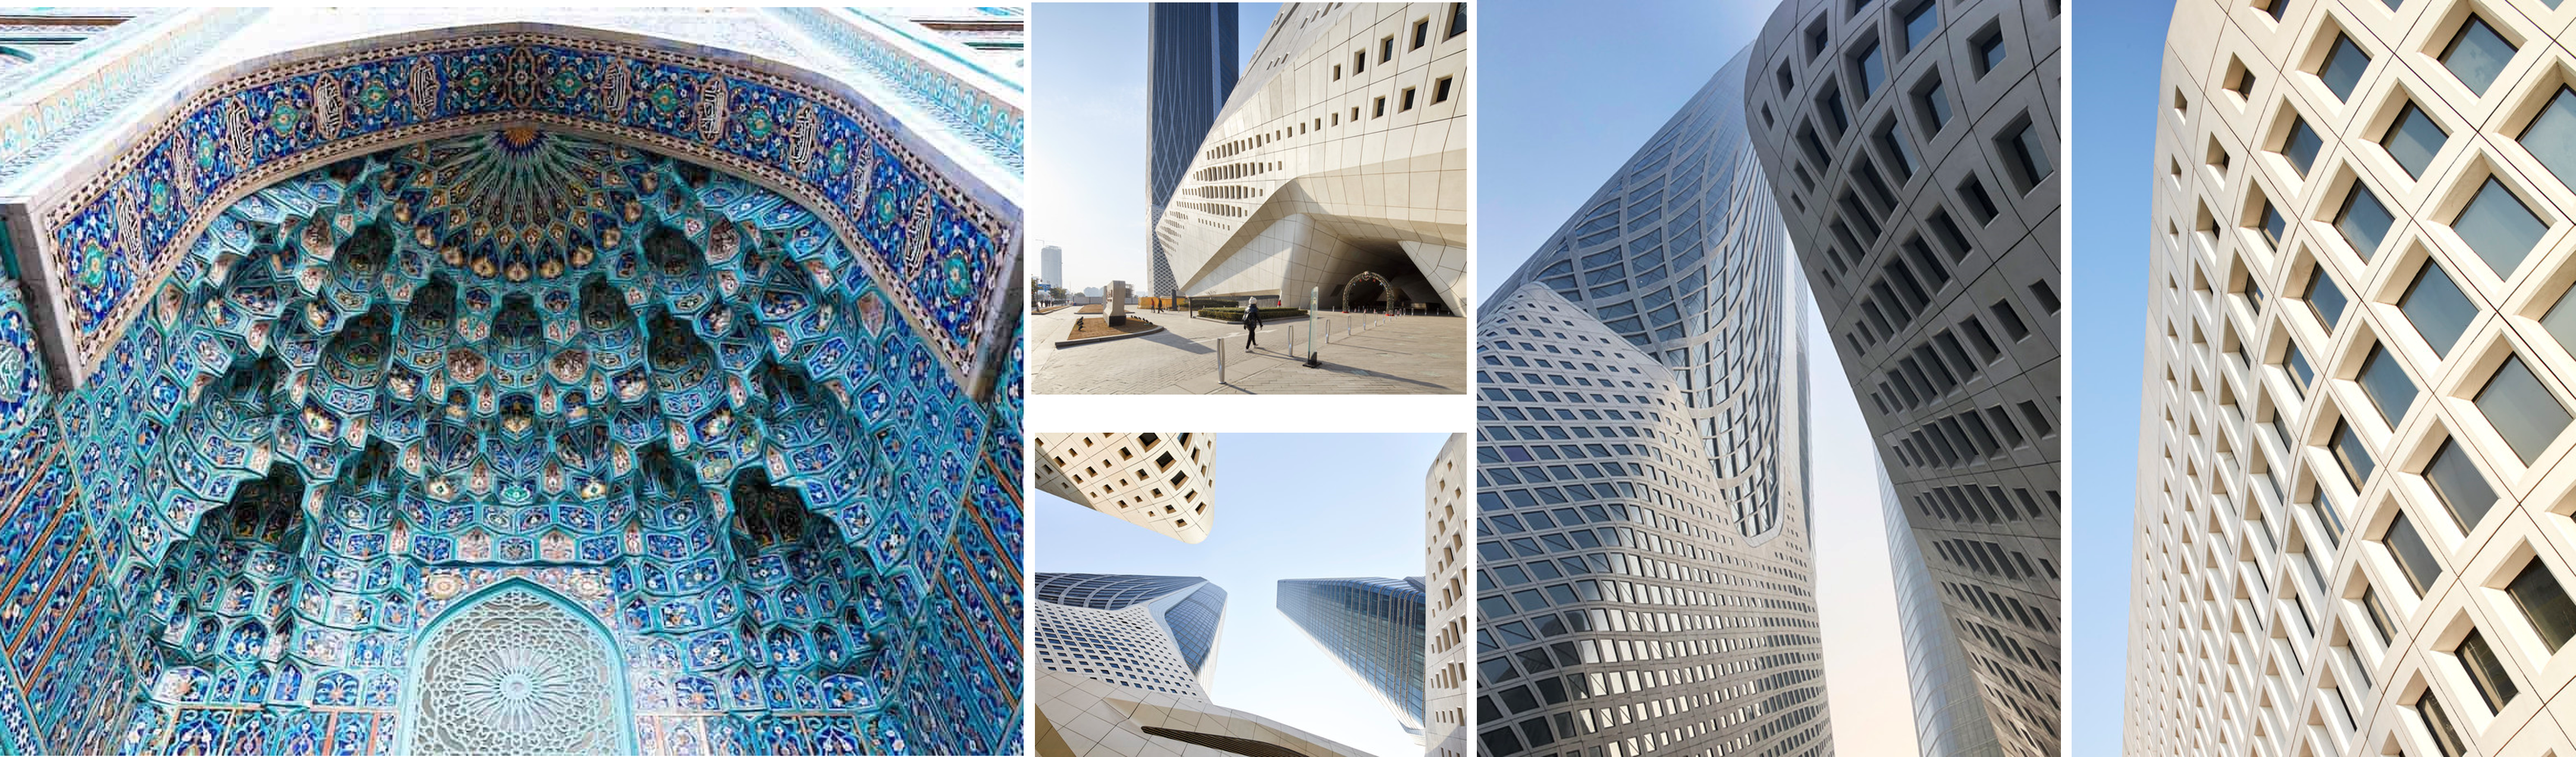
\includegraphics[width= \linewidth]{Images/complexornament}
          \caption{Complex ornament reference  (\textit{Images edited from source)}}
          \label{fig:complexornament}
        \end{figure*}


\section{Conclusions}
\label{sec:Conclusion}
%% The main conclusions of the study may be presented in a short Conclusions section, which may stand alone or form a subsection of a Discussion or Results and Discussion section.
%!%\section{Conclusions}
%%\label{sec:Conclusion}
%%%!%\section{Conclusions}
%%\label{sec:Conclusion}
%%%!%\section{Conclusions}
%%\label{sec:Conclusion}
%%\input{Text/Conclusions}

%% The main conclusions of the study may be presented in a short Conclusions section, which may stand alone or form a subsection of a Discussion or Results and Discussion section.
%% Answer the Research question

%revision

This research investigates architectural design at the intersection of digital fabrication, virtual reality (VR) assessment, and computer vision, aiming to deepen our understanding of complexity in facade design.
Our primary goal is to gauge user tolerance and acceptance of complex facades, offering insights into future construction practices.

A literature review confirmed that contemporary architecture is witnessing a trend towards increasing complexity in facade designs, moving away from the minimalist approach of the modernist movement, a trend also evidenced by the quantitative analysis across architectural history, provided by the `Computational Image Complexity Analysis' (CICA) system, which revealed an upward complexity trendline since the late 20th century (see Figure~\ref{fig:CICAscatterGraphRender}).
The historical analysis using the CICA system underscored the cultural and historical significance of facades, indicating that architectural complexity is not merely a matter of quantitative metrics but also involves cultural resonance and historical context.

Participants in the virtual reality experiment showed a preference for facades with moderate complexity, suggesting that future architectural trends may favor designs that balance intricacy with simplicity.
On average, participants favor a moderate level of complexity, with an average CICA complexity score of 3.82 (out of 10) and a 40\% probability of selecting a score close to this value according to CICA\@.

Discrepancies between participant perceptions and the CICA system's complexity rankings were particularly evident at higher complexity levels.
This highlights the subjective nature of complexity perception and the importance of integrating human feedback into architectural assessments.

The qualitative data suggests a shift towards customizable and user-responsive architectural solutions, with participants favoring form over materials and expressing a preference for facades that consider views and privacy.
This feedback suggests a strategic, view-dependent approach to facade complexity is crucial for user satisfaction.

In conclusion, this study underscores a shift in contemporary architecture towards embracing complexity in facade design, moving beyond the minimalist constraints of the modernist movement.
These insights could inform the development of nuanced and user-centric approaches in architectural design, catering to the evolving demands of modern society.


%% The main conclusions of the study may be presented in a short Conclusions section, which may stand alone or form a subsection of a Discussion or Results and Discussion section.
%% Answer the Research question

%revision

This research investigates architectural design at the intersection of digital fabrication, virtual reality (VR) assessment, and computer vision, aiming to deepen our understanding of complexity in facade design.
Our primary goal is to gauge user tolerance and acceptance of complex facades, offering insights into future construction practices.

A literature review confirmed that contemporary architecture is witnessing a trend towards increasing complexity in facade designs, moving away from the minimalist approach of the modernist movement, a trend also evidenced by the quantitative analysis across architectural history, provided by the `Computational Image Complexity Analysis' (CICA) system, which revealed an upward complexity trendline since the late 20th century (see Figure~\ref{fig:CICAscatterGraphRender}).
The historical analysis using the CICA system underscored the cultural and historical significance of facades, indicating that architectural complexity is not merely a matter of quantitative metrics but also involves cultural resonance and historical context.

Participants in the virtual reality experiment showed a preference for facades with moderate complexity, suggesting that future architectural trends may favor designs that balance intricacy with simplicity.
On average, participants favor a moderate level of complexity, with an average CICA complexity score of 3.82 (out of 10) and a 40\% probability of selecting a score close to this value according to CICA\@.

Discrepancies between participant perceptions and the CICA system's complexity rankings were particularly evident at higher complexity levels.
This highlights the subjective nature of complexity perception and the importance of integrating human feedback into architectural assessments.

The qualitative data suggests a shift towards customizable and user-responsive architectural solutions, with participants favoring form over materials and expressing a preference for facades that consider views and privacy.
This feedback suggests a strategic, view-dependent approach to facade complexity is crucial for user satisfaction.

In conclusion, this study underscores a shift in contemporary architecture towards embracing complexity in facade design, moving beyond the minimalist constraints of the modernist movement.
These insights could inform the development of nuanced and user-centric approaches in architectural design, catering to the evolving demands of modern society.


%% The main conclusions of the study may be presented in a short Conclusions section, which may stand alone or form a subsection of a Discussion or Results and Discussion section.
%% Answer the Research question

%revision

This research investigates architectural design at the intersection of digital fabrication, virtual reality (VR) assessment, and computer vision, aiming to deepen our understanding of complexity in facade design.
Our primary goal is to gauge user tolerance and acceptance of complex facades, offering insights into future construction practices.

A literature review confirmed that contemporary architecture is witnessing a trend towards increasing complexity in facade designs, moving away from the minimalist approach of the modernist movement, a trend also evidenced by the quantitative analysis across architectural history, provided by the `Computational Image Complexity Analysis' (CICA) system, which revealed an upward complexity trendline since the late 20th century (see Figure~\ref{fig:CICAscatterGraphRender}).
The historical analysis using the CICA system underscored the cultural and historical significance of facades, indicating that architectural complexity is not merely a matter of quantitative metrics but also involves cultural resonance and historical context.

Participants in the virtual reality experiment showed a preference for facades with moderate complexity, suggesting that future architectural trends may favor designs that balance intricacy with simplicity.
On average, participants favor a moderate level of complexity, with an average CICA complexity score of 3.82 (out of 10) and a 40\% probability of selecting a score close to this value according to CICA\@.

Discrepancies between participant perceptions and the CICA system's complexity rankings were particularly evident at higher complexity levels.
This highlights the subjective nature of complexity perception and the importance of integrating human feedback into architectural assessments.

The qualitative data suggests a shift towards customizable and user-responsive architectural solutions, with participants favoring form over materials and expressing a preference for facades that consider views and privacy.
This feedback suggests a strategic, view-dependent approach to facade complexity is crucial for user satisfaction.

In conclusion, this study underscores a shift in contemporary architecture towards embracing complexity in facade design, moving beyond the minimalist constraints of the modernist movement.
These insights could inform the development of nuanced and user-centric approaches in architectural design, catering to the evolving demands of modern society.


\section{Declaration of Competing Interest}
\label{sec:DeclarationInterest}
%% Declaration of using AI to edit the text
\input{Text/DeclarationInterests}

%\section{Declaration of generative AI and AI-assisted technologies in the writing process}
%\label{sec:Declaration AI}
%% Declaration of using AI to edit the text
%%%Declaration of generative AI and AI-assisted technologies in the writing process

During the preparation of this work, the author(s) used CHAT GPT/ OPEN AI in order to improve language and readability.
After using this tool/service, the author(s) reviewed and edited the content as needed and take(s) full responsibility for the content of the publication.

%% End of line numbers
\end{linenumbers}

%% If you have bibdatabase file and want bibtex to generate the
%% bibitems, please use
%%
%\newpage
%\clearpage
\bibliographystyle{elsarticle-num}
\bibliography{main}

%% The Appendices part is started with the command \appendix;
%% appendix sections are then done as normal sections
\newpage
\clearpage
\appendix

\section{Survey}
\label{sec:Annexsurvey}
The evaluation survey had two sections.
The first one tasked with identifying the professional background of the participants (see Table\ref{tab:BackgroundSurvey}).
The second one, a 10 question survey using a 7-point Likert scale to measure the degree of complexity and pattern arrangement within facade design  tailored for digital fabrication (see Table\ref{tab:ComplexitySurvey}).

%% Participant background section table from survey
    \begin{table}[htb]
        \centering
        \footnotesize
        \caption{Multiple choice survey for professional background}
        \label{tab:BackgroundSurvey}
        \begin{tabularx}{\linewidth}{p{0.125cm}X}
            \toprule
            & \textit{Participant background section. Multiple choice questions} \\
            \midrule
            1 & What is your current occupation? \\
            & a) Architect \\
            & b) Civil engineer \\
            & c) Construction manager \\
            & d) Urban planner \\
            & e) Other (please specify) \\
            \addlinespace
            2 & How many years of professional experience do you have in facade design? \\
            & a) None \\
            & b) Less than 1 year \\
            & c) 1--5 years \\
            & d) 6--10 years \\
            & e) More than 10 years \\
            \addlinespace
            3 & What is the highest level of education you have completed? \\
            & a) High school diploma \\
            & b) Associate degree \\
            & c) Bachelor's degree \\
            & d) Master's degree \\
            & e) Doctoral degree \\
            \addlinespace
            4 & Which software tools have you used for facade design? (Select all that apply) \\
            & a) AutoCAD \\
            & b) SketchUp \\
            & c) Revit \\
            & d) Rhino \\
            & e) ArcGIS \\
            & f) Other (please specify) \\
            \addlinespace
            5 & What challenges have you encountered when designing facades? (Select all that apply) \\
            & a) Limited space \\
            & b) Limited budget \\
            & c) Building program constraints \\
            & d) Client preferences \\
            & e) Environmental factors \\
            & f) Other (please specify) \\

            \bottomrule

        \end{tabularx}
    \end{table}

%% Complexity perception section table from survey
    \begin{table}[htb]
        \centering
        \footnotesize
        \caption{Complexity perception section  from survey for complexity analysis for facade design design}
        \label{tab:ComplexitySurvey}
        \begin{tabularx}{\linewidth}{p{0.125cm}X}
            \toprule
            & \textit{Complexity perception section. 7 - Likert scale} \\
            \midrule
            6 & To what extent do you find the overall complexity of this facade design appealing?\\
            & Strongly Disagree (1) —————— Strongly Agree (7) \\
            \addlinespace
            7 & How do you rate the intricacy of the patterns and textures used in this facade design? \\
            & Not Intricate at All (1) —————— Extremely Intricate (7)\\
            \addlinespace
            8 & To what extent do you think the arrangement of architectural elements on this facade adds to its visual interest? \\
            & Not at All (1) —————— Adds Significantly (7) \\
            \addlinespace
            9 & How complex do you perceive the facade's use of patterns and textures? \\
            & Not Complex at All (1) —————— Very Complex (7) \\
            \addlinespace
            10 & How detailed do you find the ornamentation on this facade design? \\
            & Not Detailed at All (1) —————— Extremely Detailed (7) \\
            \addlinespace
            11 & How much do the combination of materials contribute to the overall complexity of the facade? \\
            & Minimally (1) —————— Significantly (7) \\
            \addlinespace
            12 & To what degree does the composition of the facade strike you as aesthetically intricate? \\
            & Not Intricate at All (1) —————— Extremely Intricate (7) \\
            \addlinespace
            13 & How much do you believe that the arrangement of shapes and forms on the facade contributes to its complexity? \\
            & Not at All (1) —————— A Great Deal (7) \\
            \addlinespace
            14 & How significantly does the use of color enhance the facade's visual complexity? \\
            & Not Significantly (1) —————— Very Significantly (7) \\
            \addlinespace
            15 & How much depth and layering do you observe in the design of this facade? \\
            & None (1) —————— A Great Deal (7) \\
            \bottomrule
        \end{tabularx}
    \end{table}


\section{Pattern Variations}
\label{sec:AnnexVariations}
\input{Text/AnnexVariations}

\end{document}